\documentclass[11pt]{article}

\usepackage[T2A]{fontenc}
\usepackage[utf8]{inputenc}
\usepackage[english]{babel}
\usepackage{amssymb}
\usepackage{amsmath}

\usepackage[colorlinks=true]{hyperref}
%\usepackage[top=2cm,bottom=2cm,left=2cm,right=2cm]{geometry}

\usepackage{amsthm}
\newtheorem{theorem}{Theorem}[section]
\newtheorem{definition}{Definition}[section]

%\newenvironment{proof}[1][Proof]{\begin{trivlist}
%\item[\hskip \labelsep {\bfseries #1}]}{\end{trivlist}}
%\newenvironment{definition}[1][Definition]{\begin{trivlist}
%\item[\hskip \labelsep {\bfseries #1}]}{\end{trivlist}}
%\newenvironment{theorem}[1][Theorem]{\begin{trivlist}
%\item[\hskip \labelsep {\bfseries #1}]}{\end{trivlist}}
%\newenvironment{example}[1][Example]{\begin{trivlist}
%\item[\hskip \labelsep {\bfseries #1}]}{\end{trivlist}}
%\newenvironment{remark}[1][Remark]{\begin{trivlist}
%\item[\hskip \labelsep {\bfseries #1}]}{\end{trivlist}}
%
%\newcommand{\qed}{\nobreak \ifvmode \relax \else
%      \ifdim\lastskip<1.5em \hskip-\lastskip
%      \hskip1.5em plus0em minus0.5em \fi \nobreak
%      \vrule height0.75em width0.5em depth0.25em\fi}

\usepackage{enumitem}
\usepackage{multirow}
\usepackage{longtable}
\usepackage{afterpage}

\usepackage{subfig}
\usepackage{graphicx}
\graphicspath{ {./imgs/} }

\DeclareMathOperator{\Tr}{Tr}


\begin{document}

\section{Introduction}
One of the foundations of classical mechanics is a principle of local realism. Locality stands that any object can be affected only by its nearest local space and there is no action that can be transmitted faster than the light speed. Realism refers to a philosophical position that the observed values are properties of objects, that is, they are objective and can be attributed to physical systems before the measurement. These postulates are not only confirmed by classical physical experiments, intuitively they are plausible assumptions on the real world.

However, modern quantum mechanics is questioning the adequacy of the model of local realism to the description of the microcosm. According to the Heisenberg uncertainty principle there is a fundamental limit of the accuracy for the joint measurement of the coordinate of a quantum particle and its momentum (as well as any other joint measurement of two observables, described by non-commuting operators). It means that for a quantum system, the values of position and momentum cannot be be assigned to it before measurement. Thus, as a consequence of the Heisenberg principle, in quantum world there is no place for realism.

However, his position was criticised by Einstein, Podolsky and Rosen(EPR paradox)\cite{EPR}. They showed using quantum mechanics formalism that it is possible to come to the contradiction with the above principle. They presented a hypothetical experiment in which one can accurately determine the position and momentum of a particle, taking measurements for particles in the entangled state, located far enough from each other. The discussion of this paradox raised the question of possible incompleteness of the quantum theory. Perhaps, quantum mechanics does not completely describe the state of the system, and there are still some unknown hidden parameters. Another explanation of the paradox is the rejection of the locality principle.

Further evidence of contradiction between classical and quantum models of real world was given by Bell and other authors in the form of statistical inequalities which can be tested experimentally. At the very beginning the question about the existence of locality and realism seemed to be a philosophical discussion about the nature of the reality, but after it was formulated using mathematical formalism and then tested experimentally. Despite the fact that violations of Bell inequalities predicted by quantum mechanics, were observed in the most of experiments \cite {ASP1}, the process of verification is still not completed \cite {Khrennikov_preprint}.

The main reason of further tests is that as any experiment, Bell's test cannot be performed with 100\% efficiency of detectors and without any noise in the detector response. An example of inequality that takes into account these types of errors, is an Eberhard's inequality that was presented in the article \cite{Eberhard}. On its basis a number of experiments such as \cite{Zeilinger} was conducted, which also revealed the violation of the predictions of the classical theory.

The main difficulty in such experiments is that violations of inequality require a fairly high efficiency of detectors, special initial state of a quantum system and installation angles of polarization beam splitters. These parameters should be such that the inequality is violated as much as possible. To achieve this result Eberhard used a simple brute-force optimization.

This work is devoted to mathematical modeling of parameters of the Eberhard's inequality using optimization techniques. The main purpose is to consider more general case when the detectors have different efficiencies. In addition, in the article \ cite {Eberhard} the objective function has the sense of mathematical expectation. However, it is also useful to investigate the possible level of variability of the results, expressed in terms of standard deviation. In this paper we consider the optimization of parameters for the Eberhard's inequality using coefficient of variation taking into account possible errors in the setup of angles during the experiment.


\section{Required elements of functional analysis}
\subsection{Hilbert space and linear operator on it}
Here we present some basic definitions of function analysis which can be used in quantum mechanics formalism. Our presentation will be brief and not detailed, see, e.g. \cite{advanced_la}, for details.

\begin{definition}
For the complex vector space $V$ inner (scalar) product $\langle\cdot,\cdot\rangle$ is a map $V\times V \to \mathbb{C}$ that satisfies conditions:
\begin{enumerate}
\item Conjugate symmetry - $\langle x, y\rangle = \overline{\langle y, x\rangle}$,
\item It is positively defined - $\langle x, y\rangle \geq 0$ and $\langle x, y\rangle = 0 \Leftrightarrow x = y$,
\item Linearity - $\langle x, ay\rangle = a\langle x, y\rangle$ where $a\in\mathbb{C}$, and $\langle x, y_1 + y_2\rangle = \langle x, y_1\rangle + \langle x, y_2\rangle$.
\end{enumerate}
\end{definition}

\begin{definition}
Hilbert space $H$ is a complex vector space with an inner product which is complete with respect to the norm $\|x\| = \sqrt{\langle x, x\rangle}$
\end{definition}

The space $H = \mathbb{C}^n$ with an inner product defined by $\langle\psi, \varphi \rangle = \sum_{i = 1}^n \overline{\psi_i}\varphi_i$. Another well-known example is the functional space $H = L_2(\mathbb{R}^n, dx)$ of square integrable function with respect to the Lebegue measure. In this space inner product is defined by $\langle\psi, \varphi \rangle = \int_{\mathbb{R}^n}\overline{\psi(x)}\varphi(x) dx$.

Another important notion which is widely used in quantum mechanics theory is the notion of a linear operator.
\begin{definition}
Linear operator $A$ on a Hilbert space $H$ is a map $H \to H$ that has the following properties:
\begin{enumerate}
\item $\forall \psi_1,\psi_2\in H: A(\psi_1 + \psi_2) = A\psi_1 + A\psi_2 $
\item $\forall\lambda\in\mathbb{C}, \psi\in H: A(\lambda\psi) = \lambda A\psi$
\end{enumerate}
\end{definition}

Let us assume that Hilbert space has finite dimension to simplify further considerations.

\begin{definition}
For a linear operator $A$, its adjoint operator $A^*$ is denoted with the aid of the equality $\langle A\psi,\varphi\rangle = \langle\psi, A^*\varphi\rangle$. Operator $A$ is called self-adjoint if $A^* = A$.
\end{definition}

\begin{definition}
Let $V$ be a vector space over $\mathbb{C}$ and let $A$ be an operator on $V$.
\begin{enumerate}
\item A scalar $\lambda\in \mathbb{C}$ is an eigenvalue of $A$ if there exists a nonzero vector $\psi\in V$ for which
\[
A\psi = \lambda\psi.
\]
\item Such a vector $\psi$ is called an eigenvector of $A$.
\item In some cases there are several different eigenvectors associated with the same eigenvalue $\lambda$. They together with the zero vector form a subspace of $V$ called the eigenspace of $\lambda$.
\item The set of all eigenvalues of an operator is called the spectrum.
\end{enumerate}
\end{definition}

For self-adjoint operators in Hilbert space the following theorem holds.
\begin{theorem}
For every self-adjoint operator $A$ in complex Hilbert space $H$:
\begin{enumerate}
\item All its eigenvalues are real,
\item In $H$ there is an orthonormal basis consisting of its eigenvectors.
\end{enumerate}
\end{theorem}

\begin{definition}
A self-adjoint bounded operator is called positive if it has only non-negative eigenvalues in its spectrum.
\end{definition}

Another useful operator on Hilbert space is a projector operator.
\begin{definition}
Let $H_0$ be a linear subspace of $H$. Operator $\pi: H \to H - H_0$ is called a projector if $\pi^* = \pi$ and $\pi^2 = \pi$. It projects $H$ orthogonally onto $H_0 = \pi(H)$.
\end{definition}
Let $\{e_1, \ldots, e_n\}$ be a basis in $H$ and $\{e_1, \ldots e_m\}$ a basis in $H_0$. If $e_j \in H_0$ then $\pi e_j = e_j$ and if $e_j\in H_0^\perp$ then $\pi e_j = 0$. For an arbitrary element $\psi\in H$, the projector operator acts as: 
\[
\pi\psi = \sum_{i = 1}^m z_ie_i, \mbox{ where } z_i = \langle e_i, \psi\rangle.
\]

\subsection{Tensor product}
Let $H_1$ be a vector space with an orthogonal basis system $\{e_1, \ldots e_n\}$ and let $H_2$ be another vector space with an orthogonal basis $\{f_1,\ldots f_m\}$. We will use formal symbol $\otimes$ to construct a new orthogonal basis from the set of ordered pairs $(e_i, f_j)$ in a new vector space:
\begin{equation}
\{e_i \otimes f_j | e_i \in H_1, f_j \in H_2\}. \label{eq:tensor_basis}
\end{equation}

\begin{definition}
The set of formal sums of the form
\begin{equation}
\psi = \sum_{i,j}z_{i,j}e_i\otimes f_j,\ z_{i,j} \in \mathbb{C}
\label{eq:tensor_element}
\end{equation}
with naturally defined operation of addition and multiplication by scalar is called the tensor product of $H_1$ and $H_2$ and denoted by the symbol $H = H_1\otimes H_2$
\end{definition}

If $H_1$ and $H_2$ are Hilbert spaces then $H = H_1\otimes H_2$ is also Hilbert space with the inner product defined by
\[
\langle\psi, \varphi\rangle = \langle \sum_{i,j}z_{i,j}e_i\otimes f_j, \sum_{k,l}v_{k,l}e_k\otimes f_l \rangle = \sum_{i, j}\sum_{k, l}\overline{z_{i,j}}v_{k,l} \langle e_i\otimes f_j, e_k\otimes f_l \rangle,
\]
where a scalar product of basis vectors is defined by
\[
\langle e_i\otimes f_j, e_k\otimes f_l \rangle \overset{\mbox{def}}= \langle e_i, e_k\rangle \cdot \langle f_j, f_l \rangle = \delta_{i, k}\delta_{j, l}.
\]

For the elements $\psi_1, \psi_2$ from spaces $H_1$ and $H_2$, correspondingly, the tensor product is given by
\begin{equation}
\psi_1 \otimes \psi_2 = \left(\sum_ix_ie_i\right) \otimes \left(\sum_jy_jf_j\right) \overset{\mbox{def}}= \sum_{i, j} x_iy_j \cdot e_i \otimes f_j \in H_1 \otimes H_2.
\label{eq:tensor_factorizable}
\end{equation}
Elements of $H = H_1\otimes H_2$ which can be written in the form \eqref{eq:tensor_factorizable} are called factorizable elements. But space $H$ does not consist only of factorizable elements. Here we construct an example of a vector that cannot be written in the form  \eqref{eq:tensor_factorizable}.

Consider Hilbert space $H_1\otimes H_2$, where $H_i$ are Hilbert spaces with the basis $\{e_1, e_2\}$. Let us show that the following quantum state $\psi$ is not factorizable
\[
	\psi = \frac{e_1 \otimes e_2 + e_2 \otimes e_1}{2} \ne \psi_1 \otimes \psi_2
\]
for any pair $\psi_1, \psi_2$.
\begin{proof}
Let assume that $\psi$ can be represented as $\psi = \psi_1\otimes\psi_2$ where
$\psi_1$ and $\psi_2$ can be written as weighted sums of basis vectors:
\begin{gather*}
	\psi_1 = a_1 e_1 + a_2 e_2,\ a_i\in \mathbb{C},\ |a_1|^2 + |a_2|^2 = 1 \\
	\psi_2 = b_1 e_1 + b_2 e_2, b_i\in \mathbb{C}, |b_1|^2 + |b_2|^2 = 1.
\end{gather*}
Such a $\psi$ can be represented as
\begin{eqnarray*}
	\psi_1 \otimes \psi_2 &=& (a_1 e_1 + a_2 e_2) \otimes (b_1 e_1 + b_2 e_2) = \\ &=&  
	a_1 b_1 \cdot e_1 \otimes e_1 + a_1 b_2 \cdot e_1 \otimes e_2 + 
	a_2 b_1 \cdot e_2 \otimes e_1 + a_2 b_2 \cdot e_2 \otimes e_2.
\end{eqnarray*}
One should solve the following system of equations to find coefficients $a_1$, $a_2$, $b_1$, $b_2$:
$$
\begin{cases}
a_1 b_2 = \frac12 \\
a_2 b_1 = \frac12 \\
a_1 b_1 = 0 \\
a_2 b_2 = 0
\end{cases}
$$
which is inconsistent. Therefore $\psi$ is not factorizable.
\end{proof}
 
\begin{definition}
Consider two linear operators $A_1: H_1\to H_1$ and $A_2: H_2\to H_2$. The tensor product of these operators is defined by the equality
\[
(A_1\otimes A_2)(\psi_1\otimes \psi_2) = A_1\psi_1 \otimes A_2\psi_2.
\]
%In case of operators $A_1, A_2$ are written in a matrix form as $A^1, A^2$ correspondingly their tensor product is defined by a Kronecker product of two matrices:
%\[
%A_1\otimes A_2 = 
%\begin{pmatrix}
%a^1_{1,1}\cdot A^2 & \ldots & a^1_{1,n}\cdot A^2\\
%\ldots & \ldots & \ldots\\
%a^1_{n,1}\cdot A^2 & \ldots & a^1_{n,n}\cdot A_2
%\end{pmatrix}.
%\]
\end{definition}


%\subsection{Generalized functions}
%The concept of generalized function is the extension to the notion of  functions. Here we present a description of it from \cite{gelfand}.
%
%\begin{definition}
%Bump function - is a real-valued function $f$ which has continuous derivatives of all orders and equals to zero outside some bounded region(has compact support).
%\end{definition}
%Consider the set of such functions $K$. Assume that the sequence of bump functions $\varphi_1,\varphi_2\ldots$ tends to zero in the $K$ space if all of this functions equal to zero outside the same bounded region and each sequence of them and their derivatives tends uniformly to zero.
%
%One of the examples of such functions is the sequence $\varphi_\nu(x) = \frac{1}{\nu}\varphi(x, a)$ where 
%\[
%\varphi(x, a) = \left\{
%\begin{aligned}
%&e^{-\frac{a^2}{a^2 - x^2}},&\ x<a\\
%&0,&\ \mbox{otherwise}\\
%\end{aligned} \right. .
%\]
%It and all its derivatives uniformly tend to zero and all function in the sequence become zero in the region where $x \geq a$.
%
%\begin{definition}
%We are given a generalized function $f$ if there is a rule according to which for every bump function $\varphi$ we have a mapping to the a number $(f, \varphi)$ that satisfies following conditions:
%\begin{enumerate}
%\item Linearity - $(f, \alpha_1\varphi_1 + \alpha_2\varphi_2) = (f, \alpha_1\varphi_1) + (f, \alpha_2\varphi_2)$;
%\item Continuity - if some sequence of bump functions $\varphi_1,\varphi_2,\ldots$ tends to zero in the space $K$ then the sequence of numbers $(f, \varphi_1), (f, \varphi_2), \ldots$ converges to zero in $\mathbb{R}$.
%\end{enumerate}
%\end{definition}
%
%For example, consider a function $f$ which is absolutely integrable in every finite region of $\mathbb{R}^n$. With this function for every bump function $\varphi$ we can map a number 
%\begin{equation}
%(f, \varphi) = \int_{\mathbb{R}^n} f(x)\varphi(x) dx. \label{eq:non-singular-generalized}
%\end{equation}
%
%Another example of generalized function is Dirac delta function $\delta(x)$:
%\begin{equation}
%(\delta, \varphi) = \int_{-\infty}^{+\infty} \delta(x)\varphi(x) dx = \varphi(0). \label{eq:delta-function}
%\end{equation}
%
%Generalized functions that cannot be represented in the form \eqref{eq:non-singular-generalized} called singular. Delta function is an example of singular functions.
%
%\subsection{Dirac delta function and its properties}
%
%Every singular function can be represented as a limit a sequence of nonsingular generalized functions.
%\begin{definition}
%The sequence of generalized functions $f_1, f_2,\ldots f_\nu,\ldots$ converges to generalized function $f$ if
%\[
%\lim_{\nu\to\infty} (f_\nu, \varphi) = (f, \varphi).
%\]
%\end{definition}
%
%Dirac delta function \eqref{eq:delta-function} can be defined as a limit of nonsingular functional sequence $f_\nu$ with the following properties:
%\begin{enumerate}
%\item $\forall M > 0:\ \forall a, b\ |a| \leq M,\ |b| \leq M$ integral 
%\[
% \left| \int_a^b f_\nu(\xi)d\xi \right| \leq C(M)
%\]
%\item for every fixed $a, b > 0$
%\[
%\lim_{\nu\to\infty} \int_a^bf_\nu(\xi)d\xi = \left\{
%\begin{aligned}
%&0,&\ a < b < 0 \mbox{ or } 0 < a < b,\\
%&1,&\ a < 0 < b\\
%\end{aligned} \right. .
%\]
%\end{enumerate}
%One example of such functions is the sequence 
%\[
%f_\epsilon(x) = \dfrac{1}{\pi} \dfrac{\epsilon}{x^2 + \epsilon^2}
%\]
%where $\epsilon\to 0$.
%
%Delta function has some useful properties:
%\begin{enumerate}
%\item $\int _{-\infty}^{+\infty} f(x)\delta(x - x_0)dx = f(x_0)$,
%\item $\delta\left(\dfrac{x}{a}\right) = |a|\delta(x)$,
%\item another way to define $\delta(x)$ is to compute its Fourier transformation using \eqref{eq:delta-function}:
%\[
%\tilde{\delta}(\omega) = \int_{-\infty}^{+\infty}\dfrac{e^{i\omega t}}{\sqrt{2\pi}}\delta(t)dt = \dfrac{1}{\sqrt{2\pi}}.
%\]
%From the above equation one can find that 
%\[
%\delta(t) = \int_{-\infty}^{+\infty}\dfrac{e^{-i\omega t}}{\sqrt{2\pi}}\tilde{\delta}(\omega)d\omega = \int_{-\infty}^{+\infty}\dfrac{e^{-i\omega t}}{2\pi}d\omega.
%\]
%This equation can be used as another form of defining dirac delta function.
%\end{enumerate}
%

\section{Mathematical formalism of quantum mechanics}
\subsection{Postulates of quantum mechanics }
The mathematical formalism of quantum mechanics can be formulated as a list of postulates \cite{Khrennikov_information} which are based on the theory of self-adjoint operator on complex Hilbert space $H$. The following list of postulates and principles is called Copenhagen interpretation of quantum mechanics.
\begin{enumerate}[label=\bfseries Postulate \arabic*:, align=left]
  \item A quantum state $\psi$ is a vector of a complex Hilbert space such that $\langle\psi, \psi\rangle = 1$. This vector completely describes the state of a quantum system. Two vectors which differ by a factor of $\gamma = e^{i\varphi}$ describe the same quantum state.
  \item A physical observable $a$ is represented as a self-adjoint operator $A$ in $H$. Different observables are represented by different operators.
  \item If an observable is represented by the operator $A$ then results of observation are given by the spectrum of $A$. Any self-adjoint operator can be written in the form 
  \[
  A = \sum_m a_m\pi_m^A
  \]
    where $\pi_m^A$ is an orthogonal projector onto an eigenspace corresponding to the eigenvalue $a_m$.
  \item Born's rule - if $A$ is a self-adjoint operator then the probability to obtain an eigenvalue $a_m$ after measurement can be calculated by using the formula
  \[
  P(a = a_m) = \| \pi_m^A\psi\|^2.
  \]
  \item 
  Consider a quantum state $\psi$ and a self-adjoint operator $A$. Eigenvectors of $A$ with its eigenvalues $\{a_m\}$ form a basis in the Hilbert space $H$: $\{ \varphi: A\varphi = a_m\varphi\}$ so this state can be represented as $H = H_1\oplus H_2\oplus\ldots H_k$. Projector $\pi_m^A: H\to H_m$ equals to 
  \[
  \pi_m^A = \sum_{l = 1}^{n_m}\langle\psi,\varphi_{ml}\rangle\varphi_{ml}
  \]
  where $\varphi_{ml}$ - $l$-th eigenvector from $H_m$.
  Then quantum state of a system collapses to state $\psi_m$:
  \[
  \psi_m = \frac{\pi_m^A\psi}{ \| \pi_m^A\psi\|}
  \] 
  after a measurement with a result $A \to a_m$.
  \item The time evolution of the quantum state $\psi$ satisfies the Schr\"{o}dinger equation
  \[
  i\hbar \dfrac{d}{dt}\psi(t) = \mathcal{\mathcal{H}}\psi(t)
  \] 
  with the initial condition $\psi(0) = \psi_0$ and
  where $\mathcal{H}$ is a self-adjoint positive operator representing the energy of the system.
  \item If there are two quantum systems int Hilbert spaces $H_1$ and $H_2$, then the state space of the compound system is given by $H_1 \otimes H_2$.  
\end{enumerate}
\begin{definition}
If a state $\psi\in H_1\otimes H_2$ is not factorizable in the form $\psi = \psi_1\otimes\psi_2$ where $\psi_1\in H_1, \psi_2\in H_2$ then it is called entangled.
\end{definition}  
Consider Hilbert 2-dimensional spaces $H_1 = H_2$ the basis $\{e_1, e_2\}$. One of the examples of entanglement is 
\[
\psi = \frac{e_1\otimes e_2 + e_2\otimes e_1}{2}.
\]
It was shown before that in that state $\psi$ cannot be factorizable as $\psi = \psi_1\otimes\psi_2$.

Another example is $\psi = e_1\otimes e_2 + e_1 \otimes e_1 + 2e_2 \otimes e_1$.

\begin{proof}
Let us assume that $\psi$ is represented in the form $\psi = \psi_1\otimes\psi_2$, where $\psi_1$ and $\psi_2$ can be written as a weighted sum of basis vectors:
\begin{gather*}
	\psi_1 = a_1 e_1 + a_2 e_2,\ a_i\in \mathbb{C},\ |a_1|^2 + |a_2|^2 = 1 \\
	\psi_2 = b_1 e_1 + b_2 e_2, b_i\in \mathbb{C}, |b_1|^2 + |b_2|^2 = 1.
\end{gather*}
For this $\psi$ one can construct that:
\begin{eqnarray*}
	\psi_1 \otimes \psi_2 &=& (a_1 e_1 + a_2 e_2) \otimes (b_1 e_1 + b_2 e_2) = \\ &=&  
	a_1 b_1 \cdot e_1 \otimes e_1 + a_1 b_2 \cdot e_1 \otimes e_2 + 
	a_2 b_1 \cdot e_2 \otimes e_1 + a_2 b_2 \cdot e_2 \otimes e_2.
\end{eqnarray*}
One should solve the following system of equations to find coefficients $a_1$, $a_2$, $b_1$, $b_2$:
$$
\begin{cases}
a_1 b_2 = \frac{1}{\sqrt{6}} \\
a_2 b_1 = \frac{2}{\sqrt{6}} \\
a_1 b_1 = \frac{1}{\sqrt{6}} \\
a_2 b_2 = 0
\end{cases},
$$
which is inconsistent. Therefore the assumption is false and $\psi$ is not factorizable.
\end{proof}


\subsection{Density operator}

To describe a behaviour of an ensemble of quantum states where each state is obtained with some probability we will use the notion of a density operator from \cite{Khrennikov_information}.

For a pure state $\psi$ we can define an orthogonal projection operator: $P_\psi: P_\psi\varphi = \langle \psi, \varphi \rangle \psi$. It has following properties:
\begin{enumerate}
\item $P_\psi$ is hermitian. 
\begin{proof}
$\langle P_\psi\varphi, v\rangle = \langle \langle\psi,\varphi\rangle \psi, v\rangle = \overline{\langle\psi,\varphi\rangle} \langle\psi, v\rangle = \langle\psi, v\rangle \langle\varphi,\psi\rangle  = \langle\varphi, \langle\psi, v\rangle\psi\rangle = \langle\varphi, P_\psi v \rangle$
\end{proof}
\item $P_\psi \geq 0$.
\begin{proof}
$\langle P_\psi\varphi, \varphi\rangle = \overline{\langle\psi,\varphi\rangle} \langle\psi, \varphi\rangle = |\langle\psi, \varphi\rangle|^2 \geq 0$
\end{proof}
\item $\Tr P_\psi = 1$ where $\Tr A = \sum_k \langle Ae_k, e_k\rangle$ and $\{e_k\}$ is an orthogonal basis.
\begin{proof}
$\Tr P_\psi = \sum_{k = 1}^n \langle \langle \psi, e_k\rangle\psi, e_k\rangle = \sum_k \overline{\langle\psi, e_k\rangle}\langle\psi, e_k\rangle = \sum_k\psi_k^2 = 1$
\end{proof}
\item $P_\psi^2 = P_\psi$
\begin{proof}
$P_\psi^2\varphi = \langle\psi, \langle\psi, \varphi\rangle \psi\rangle \psi = \langle\psi, \varphi\rangle \langle\psi, \psi\rangle\psi = \langle\psi, \varphi\rangle\psi = P_\psi\varphi $
\end{proof}
\end{enumerate}
In the common case for any state or ensemble of states we can construct an operator
\[
\rho = \sum_ip_iP_{\psi_i},
\]
where $p_i > 0,\ \sum_ip_i = 1$ represents probability to obtain $\psi_i$ after a measurement.

One can easily show that operator $\rho$ satisfies properties 1-3 using corresponding properties 1-3 for each operator $P_{\psi_i}$. In the common case property 4 of projection operator is violated. For example, let us take density operator $\rho = \cfrac 12P_{\psi_1} + \cfrac 12P_{\psi_2}$ where $\psi_1 = (1, 0)^T$ and $\psi_2 = (0, 1)^T$. Let us find the square of this operator:
\[
\rho^2\varphi = \frac 12\langle\psi_1, \rho\varphi\rangle\psi_1 + \frac 12\langle\psi_2, \rho\varphi\rangle\psi_2 =
\]
\[
= \frac 12\langle\psi_1, \frac 12\langle\psi_1, \varphi\rangle\psi_1 + \frac 12\langle\psi_2, \varphi\rangle\psi_2 \rangle\psi_1 + \frac 12\langle\psi_2, \frac 12\langle\psi_1, \varphi\rangle\psi_1 + \frac 12\langle\psi_2, \varphi\rangle\psi_2 \rangle\psi_2 =
\]
\[
 = 
\frac 14\langle\psi_1, \langle\psi_1,\varphi\rangle\psi_1\rangle\psi_1 + \frac 14\langle\psi_1, \langle\psi_2,\varphi\rangle\psi_2\rangle\psi_1 +
\frac 14\langle\psi_2, \langle\psi_1,\varphi\rangle\psi_1\rangle\psi_2 + \frac 14\langle\psi_2, \langle\psi_2,\varphi\rangle\psi_2\rangle\psi_2
\]
The final result is:
\[
\rho^2\varphi = \frac 14 \langle\psi_1, \varphi\rangle\psi_1 + \frac 14\langle\psi_2, \varphi\rangle\psi_2 = \frac 12\rho \neq \rho.
\]


Density operator $\rho$ also can be written in the form $\rho\psi = \sum_i p_i\langle e_i, \psi\rangle e_i$. 

\subsection{Elements of quantum probability theory}
In quantum mechanics the result of a measurement depends on a state of a system that it had before it collapsed to some pure state according to the measurement result. It means that values of quantum probabilities, expectations, standard deviations etc. depend not only on an observable but also on an initial state of a system which is described by a density operator.

Let $A$ be an observable with eigenvalues $\{a_1,\ldots a_n\}$ and eigenvectors $\{f_1,\ldots f_n\}$, where $\psi$ describes the state of the system. Then the probability to obtain $a_i$ after a measurement is given by
\[
P(A = a_i) = |\langle\psi, f_i\rangle|^2 = \Tr \rho_\psi A_i
\]
where $A_i = |f_i\rangle \langle f_i|$.
\begin{proof}
$\Tr \rho_\psi A_i = \sum_j \langle\rho_\psi A_if_j, f_j\rangle = \langle \langle\rho_\psi, f_i\rangle, f_i\rangle = \langle \langle \psi, f_i\rangle\psi, f_i\rangle = $\\
$= \overline{\langle\psi, f_i\rangle} \langle\psi, f_i\rangle = |\langle\psi, f_i\rangle|^2.$
\end{proof}
For the mixture state probability by definition is given by the same formula
\[
P(A = a_i) = \Tr \rho |f_i\rangle \langle f_i|.
\]

Quantum expectation value is defined by the following formula
\[
\overline{A_\rho} \equiv \langle A\rangle = \langle A\rho, \rho\rangle = \Tr\rho A.
\]
Quantum dispersion is defined the same way as it is defined in the classical probability theory:
\[
\sigma^2_{A_\rho} = \overline{\left(A_\rho - \overline{A_\rho}\right)^2} = \overline{A^2_\rho} - \overline{A_\rho}^2.
\] 

\subsection{Heisenberg's uncertainty principle}
Uncertainty principle of quantum mechanics states that there is a limit of the precision with which some of physical parameters of one system can be known simultaneously. This limit does not depend on the precision of used measurement devices or on the level of technoloy, it is fundamental and presents in any case.

For the first time uncertainty principle was formulated by Werner Heisenberg in 1927. He discovered that the more precisely the position of a particle can be measured, the less precisely its momentum can be determined.

In 1928 it was formulated as an inequality:
\[
\sigma_x\sigma_p \geq \frac{\hbar}{2},
\]
where $\sigma_x$ is a standard deviation of position, $\sigma_p$ is a standard deviation of momentum and $\hbar$ is a Planck constant.

The most general form of uncertainty principle is given by the Schr\"{o}dinger inequality:
\begin{equation}
\sigma_A^2\sigma_B^2 \geq \left| \frac{1}{2}\langle\{A, B\}\rangle - \langle A\rangle\langle B\rangle \right|^2 + \left| \frac{1}{2i}\langle [A, B]\rangle\right|^2,
\label{eq:Schrodinger_ineq}
\end{equation}
where $[A, B] = AB - BA$ - commutator operator and $\{A, B\} = AB + BA$ - anti-commutator operator.

\begin{proof}
For the derivation of the inequality we will use Cauchy-Schwartz inequality for scalar product:
\begin{equation}
|\langle f, g\rangle |^2 \leq \langle f, f\rangle \langle g, g\rangle. \label{eq:Caushy-Schwartz}
\end{equation}

Quantum dispersion $\sigma^2_A$ of self-adjoint operator $A$ can be found using formula:
\[
\sigma_A^2 = \langle (A - \langle A\rangle)^2\psi, \psi\rangle = \langle  (A - \langle A\rangle)\psi,  (A - \langle A\rangle)\psi\rangle.
\]
We will denote $f = (A - \langle A\rangle)\psi$ and $g = (B - \langle B\rangle)\psi$, then for the left side of \eqref{eq:Caushy-Schwartz} we obtain:
\[
|\langle f, g\rangle |^2 = |\langle (A - \langle A\rangle)\psi, (B - \langle B\rangle)\psi\rangle |^2 = |\langle (B - \langle B\rangle)(A - \langle A\rangle)\psi, \psi |^2 = 
\]
\[
= | \langle BA\psi, \psi\rangle - \langle B\rangle\langle A\rangle - \langle A\rangle \langle B\rangle + \langle A\rangle\langle B\rangle |^2 = | \langle BA\rangle - \langle A\rangle\langle B\rangle |^2.
\]
As any other complex number the left side of the inequality can be written as
\[
|\langle f, g\rangle |^2 = \left| \frac{1}{2}(\langle f, g\rangle + \overline{\langle f, g\rangle})\right|^2 + \left| \frac{1}{2i}(\langle f, g\rangle - \overline{\langle f, g\rangle})\right|^2, 
\]
where $\overline{\langle f, g\rangle})$ is given by
\[
\overline{\langle f, g\rangle}) = \overline{\langle BA\psi, \psi\rangle} - \langle A\rangle\langle B\rangle = \langle\psi, BA\psi\rangle - \langle A\rangle\langle B\rangle = \langle AB\psi, \psi\rangle - \langle A\rangle\langle B\rangle.
\]
Putting it all together to the inequality \eqref{eq:Caushy-Schwartz} we have an expression from the Schr\"{o}dinger inequality \eqref{eq:Schrodinger_ineq}:
\[
\left| \frac{1}{2}(\langle BA\rangle - \langle A\rangle\langle B\rangle + \langle AB\rangle - \langle A\rangle\langle B\rangle)\right|^2 + \left| \frac{1}{2i}(\langle BA\rangle - \langle A\rangle\langle B\rangle - \langle AB\rangle + \langle A\rangle\langle B\rangle)\right|^2 \leq \sigma_A^2\sigma_B^2
\]
\[
\Leftrightarrow \left| \frac{1}{2}\langle\{A, B\}\rangle - \langle A\rangle\langle B\rangle \right|^2 + \left| \frac{1}{2i}\langle [A, B]\rangle\right|^2 \leq \sigma_A^2\sigma_B^2
\]
\end{proof}

In quantum mechanics the position operator is given by the formula:
\[
(\hat{x}f) = x\cdot f(x)
\]
and momentum operator is defined by
\[
(\hat{p}f) = \frac{\hbar}{i}\frac{df}{dx}.
\]
It the common case the Robertson inequality can be derived from \eqref{eq:Schrodinger_ineq}:
\[
\sigma_A^2\sigma_B^2 \geq \frac{1}{4}|[A, B]|^2.
\]

Commutator operator of position and momentum is 
\[
[\hat{x}, \hat{p}]f(x) = (\hat{x}\hat{p} - \hat{p}\hat{x})f(x) = x\frac{\hbar}{i}\frac{df(x)}{dx} - \frac{\hbar}{i}\frac{d xf(x)}{dx} = i\hbar If(x),
\]
where $I$ is an identity operator. Then in this case Robertson inequality becomes Heisenberg's uncertainty principle:
\[
\sigma_A^2\sigma_B^2 \geq \frac{1}{4}\hbar^2.
\]

From the derivation of Heisenberg's principle it is clear that one can construct nontrivial Robertson inequality for every operators $A$ and $B$ which have nonzero commutator. It is also clear that the result formula does not depend on technology or any conditions during measurement, it is a fundamental property of some pairs of quantum operators such as position and momentum.

\section{Einstein-Podolsky-Rosen paradox}
Einstein-Podolsky-Rosen paradox(EPR-paradox, \cite{EPR}) was published in 1935 as the criticism of some statements of the Copenhagen interpretation of quantum mechanics. The main principle of this interpretation holds that any quantum system is described as a wave-function and after measurement it collapses to one of its eigenstates with some probability. Moreover, Heisenberg's uncertainty principle stands that position of a particle and its momentum are incompatible and they cannot be measured jointly with good precision. Einstein and his colleagues did not agree with probabilistic measurement outcomes. His paper was an attempt to show some contradictions in quantum mechanics.

The article \cite{EPR} is based on a thought experiment with the following initial conditions. Consider two systems $S_1$, $S_2$, both with the state space $L_2(\mathbb{R})$ and a source which produces particles for these systems. The superposition state can be represented as a quantum state from the tensor product of its single Hilbert spaces.
Operator $A$ with eigenvalues $\{a_k\}$ and eigenvectors $\{\varphi_k(x_1)\}$ will denote an observable on $S_1$. Operator $B$  with eigenvalues $\{b_k\}$ and eigenvectors $\{\psi_k(x_1)\}$ will denote another observable on the same system. 

In the common case of two Hilbert spaces $H_1$ and $H_2$ and their basis vectors $\{e_k\}$ and $\{f_k\}$ respectively the state $\varphi = \varphi_1\otimes\varphi_2$ can be represented in the form:
\[
\varphi = \sum_{k, m}c_{k, m}e_k\otimes f_m.
\]
If $H_1 = H_2 = L_2(\mathbb{R})$ its tensor product is $L_2(\mathbb{R})\otimes L_2(\mathbb{R}) = L(\mathbb{R}^2)$. For this space such state $\varphi$ can be represented in the form
\[
\varphi (x_1, x_2) = \sum_{k, m}c_{k, m}e_k(x_1)f_m(x_2)
\]
or for the continuous case it is
\[
\varphi (x_1, x_2) = \int u(x, x_1)v(x, x_2)dx.
\]

Suppose we want to execute the measurement of $A$. Before measure the particle is in the state $\psi(x_1, x_2) = \sum_k v_k(x_2)\varphi_k(x_1)$. According to von Neumann projection postulate after measurement the system will collapse to the precise state $\psi = \varphi_m(x_1)v_m(x_2)$. It means that after measuring on $S_1$ the second system will also have determinate state $v_m(x_2)$. But in conditions where two detector are very far from each other(so they cannot have impact on each other according to locality principle) it means that the second system has to have such state $v_m(x_2)$ not only before measurement but always.

Suppose after all that we've changed our decision and we want to measure $B$ on $S_1$ instead of $A$. By analogy for the previous consideration, after measure the system will collapse to the state $\psi = \zeta_n(x_1)u_n(x_2)$ which means that in this case the second system will have state $u_n(x_2)$. And again, it has to have such state independently of the measurement on the first system i.e. it stands in this state even before any measurements.

After that thought experiments we can conclude that the second system has 2 wave-functions $v_m(x_2)$ and $u_n(x_2)$. The paradox is that we can construct such states that cannot be known simultaneously according to the Heisenberg's principle. Here we present an example from the original paper \cite{EPR}.

Consider the state $\psi(x_1, x_2) = \int e^{\frac{ip}{\hbar}(x_1+x_2-x_0)}$ where $x_0$ is a constant. On one side, it can be represented in the form $\psi(x_1, x_2) = \int\varphi(p, x_1)v(p, x_2)dp$ where $\varphi(p, x_1) = e^{\frac{ip}{\hbar}x_1}$ and $v(p, x_2) = e^{\frac{ip}{\hbar}(x_2-x_0)}$. 

Momentum operator is defined by $\hat{p} = \dfrac{\hbar}{i}\dfrac{d}{dx}$. Its eigenfunction is $\psi = e^{\frac{i\lambda}{\hbar}x}$ for eigenvalue $\lambda$. After the measure of $A$ in the first system its state will collapse to its eigenfunction $\varphi(p, x_1) = e^{\frac{ip}{\hbar}x_1}$. The state of the second system $v(p, x_2) = e^{\frac{ip}{\hbar}(x_2-x_0)}$ is an eigenfunction of momentum operator, corresponding to the eigenvalue $-p$. 

On another side considering state can be represented as $\psi(x_1, x_2) = \delta(x_1 + x_2 - x_0) = \hbar\int\delta(x - x_1)\delta (x - x_2 + x_0)dx = \int\zeta(x, x_1)u(x, x_2)dx$. 

Position operator in the second system is defined by $\hat{x_2}f = x_2f$. Its eigenfunction is $\delta(x - \lambda)$ for the eigenvalue $\lambda$. After the measure of $B$ in the first system its state will collapse to the eigenfunction $\zeta(x, x_1) = \delta(x - x_1)$. The state of the second system $u(x, x_2) = \delta(x - x_2 + x_0)$ is also an eigenfunction of position operator, corresponding to the eigenvalue $x + x_0$.

At this point authors conclude that both position and momentum in the second system are elements of reality since they couldn't be affected by measures on the first system. But Heisenberg's principle stands that they can't be known both i.e. can't be both elements of reality simultaneously. 

The question of this paradox - do quantum mechanics provide a complete description of the physical reality. But since local realism assumption is used, another explanation of this paradox can be found with rejection of the local realism.

\section{Bell inequalities}
One of possible solutions of the EPR-paradox is that the quantum mechanics theory is not complete, the actual state of a system is described not only by its quantum state $\psi$ but also by some hidden, i.e. yet unknown, variables. In this case all probabilistic predictions of quantum mechanics can be explained by existing of some unknown degrees of freedom. Using that assumption one can conclude that reality can still have deterministic nature as well as probabilistic.

John Bell in his paper \cite{Bell} assumed that there are some hidden variables $\omega$ and measurement results are random variables which depend on it. He formulated statistical inequality that contradicts with quantum mechanical predictions.

Covariance of two variables can be found using the following classical probabilistic formula:
\[
\langle \xi, \eta \rangle = \int_\Omega \xi(\omega)\eta(\omega)dP(\omega).
\]

\begin{theorem}
Consider $\xi_a(\omega)$, $\xi_b(\omega)$, $\xi_c(\omega)$ be discrete random variables which can only be equal $\pm 1$. Then the following inequality is performed:
\[
| \langle\xi_a,\xi_b\rangle -  \langle\xi_c,\xi_b\rangle | \leq 1 - \langle\xi_a,\xi_c\rangle.
\]
\end{theorem}

\begin{proof}
Using covariation formula we obtain:
\[
| \langle\xi_a,\xi_b\rangle -  \langle\xi_c,\xi_b\rangle | = \left| \int_\Omega\xi_a\xi_b dP - \int_\Omega\xi_c\xi_b dP\right| = \left|\int_\Omega (xi_a - xi_c)\xi_bdP \right|.
\]
After multiplying it by $\xi_a^2 = 1$ we have:
\[
\left|\int_\Omega (1 - \xi_a\xi_c)\xi_a\xi_bdP \right|.
\]
And finally, using that $|\xi_i| = 1$ we get the desired result:
\[
\left|\int_\Omega (1 - \xi_a\xi_c)\xi_a\xi_bdP \right| \leq  \left|\int_\Omega (1 - \xi_a\xi_c)dP\right| = 1 - \langle \xi_a\xi_c\rangle.
\]
\end{proof}

After Bell's paper some other inequalities were formulated. Wigner inequality is more suitable for testing.
\begin{theorem}
For random variables form the previous theorem the following inequality is performed:
\[
P(\xi_a = +1, \xi_b = +1) + P(\xi_b = -1, \xi_c = +1) \geq P(\xi_a = -1, \xi_c = +1).
\]
\end{theorem}

\begin{proof}
The first probability can be written as 
\[
P(\xi_a = +1, \xi_b = +1) = P(\xi_a = +1, \xi_b = +1, \xi_c = +1) + P(\xi_a = +1, \xi_b = +1, \xi_c = -1),
\]
analogously, the second one can be written as
\[
P(\xi_b = -1, \xi_c = +1) = P(\xi_a = +1, \xi_b = -1, \xi_c = +1) + P(\xi_a = -1, \xi_b = -1, \xi_c = +1).
\]
Then
\[
P(\xi_a = +1, \xi_b = +1) + P(\xi_b = -1, \xi_c = +1) = P(\xi_a = +1, \xi_b = +1, \xi_c = +1) + 
\] 
\[
 + P(\xi_a = +1, \xi_b = +1, \xi_c = -1) + P(\xi_a = +1, \xi_b = -1, \xi_c = +1) + P(\xi_a = -1, \xi_b = -1, \xi_c = +1) = 
\]
\[
 =  P(\xi_a = +1, \xi_c = +1) + P(\xi_a = +1, \xi_b = +1, \xi_c = -1) + P(\xi_a = -1, \xi_b = -1, \xi_c = +1)\geq
\]
\[
 \geq P(\xi_a = +1, \xi_c = +1).
\]
\end{proof}

Another example of an inequality of Bell type is Clauser-Horne-Shimony-Holt inequality.
\begin{theorem}
For every random variables $\xi_j(\omega)$ and $\xi'_j(\omega)$ such as $|\xi_j(\omega)| \leq 1$ and $|\xi'_j(\omega)| \leq 1$ the following inequality is performed
\[
\langle\xi_1,\xi'_1\rangle + \langle\xi_1,\xi'_2\rangle + \langle\xi_2,\xi'_1\rangle -  \langle\xi_2,\xi'_2\rangle \leq 2
\]
\end{theorem}

\begin{proof}
For real numbers bounded by 1 the following inequality holds:
\[
\xi_1\xi_1' + \xi_1\xi_2' + \xi_2\xi_1' - \xi_2\xi_2' \leq 2.
\]
After integrating it we obtain Clauser-Horne-Shimony-Holt inequality.

\end{proof}

One of the main points why Bell inequality is so interesting is that such statistical inequalities can be tested in experiments. And if classical and quantum predictions are incompatible one can check that experiment results satisfies one of predictions. But if we want to compare results of two theories we have to present a mechanism of mapping between two models. To connect quantum mechanics predictions and classical probability theory Bell made some assumptions and with them and quantum mechanic formalism these inequalities are violated. Some experiments were performed and their results also violate inequalities from the classical probability theory. 

Let us construct an example of such violation from \cite{Khrennikov_information}. Consider a two-particle system in state $\psi = \frac{1}{\sqrt{2}}(|+-\rangle - |-+\rangle)$ and a spin operator that measures a spin of one particle
\[
\sigma(\theta) = \cos\theta\sigma_z + \sin\theta\sigma_x,
\] 
where $\sigma_x$ and $\sigma_z$ - Pauli matrices:
\[
\sigma_x = 
\begin{pmatrix}
0 & 1\\
1 & 0
\end{pmatrix},\ \sigma_z = 
\begin{pmatrix}
1 & 0\\
0 & -1
\end{pmatrix}.
\]
So for the whole system operator $\sigma(\theta) \otimes I$ measures a spin of the first particle and $I \otimes \sigma(\theta)$ of the second particle.
Then
\[
P_\psi(\sigma(\theta_1) = + 1, \sigma(\theta_2) = +1) = \cos^2\frac{\theta_1 - \theta_2}{2},
\]
\[
P_\psi(\sigma(\theta_3) = + 1, \sigma(\theta_2) = -1) = \sin^2\frac{\theta_3 - \theta_2}{2},
\]
\[
P_\psi(\sigma(\theta_1) = + 1, \sigma(\theta_3) = +1) = \cos^2\frac{\theta_1 - \theta_3}{2}.
\]
In this case Wigner inequality has the form:
\[
\cos^2\frac{\theta_1 - \theta_2}{2} + \sin^2\frac{\theta_3 - \theta_2}{2} \geq  \cos^2\frac{\theta_1 - \theta_3}{2}.
\]
We take $\theta_1 = 0$, $\theta_2 = 6\theta$, $\theta_3 = 2\theta$ and we get the following inequality which is violated for some sufficiently large $\theta$:
\[
\cos^2 3\theta + \sin^2 2\theta \geq cos^2 \theta.
\]

This violation is called Bell theorem.  If this theorem is correct then quantum mechanics , or locality, or realism is wrong, as they are mutually exclusive. 

Here there are some popular interpretations of Bell's results:
\begin{enumerate}
\item Quantum mechanics is complete and nonlocal so it cannot be reduced to the classical theory.
If this interpretation is true then the state of a partial cannot be represented as random variable $\xi_a(\omega)$ so inequalities cannot be applied to the real measurements. This is the most popular interpretation.

\item Quantum mechanics is incomplete and any complete classical theory is nonlocal.
If this interpretation is true then the state of a partial cannot be represented as $\xi_a(\omega)$ because it depends of another partial $b$. The representation as $\xi_{a,b}(\omega)$ doesn't give us the same inequalities so there is no paradox between experiments and classical probability theory.

\item Some of Bell's assumptions about accordance between classical and quantum models are wrong. If this interpretation is true then there is no paradox because its proof is incorrect.
\end{enumerate}

In \cite{Khrennikov_information} it is shown that in Bell's theory there can be some incorrect assumptions in the way of accordance between classical and quantum probabilities.

Firstly, It can be contradicted that classical(an integral) and quantum equalities for covariations are equal.
$$\int_\Omega\xi_a(\omega)\xi_b(\omega)dP_\rho(\omega) \equiv Tr\rho\hat{a}\hat{b}$$
But for other variants of Bell theorem this postulate was replaced by less controversial.

Secondly, domains of classical and quantum variables can be nonequal. There are two systems - the observed and the observer. The probability measure of states for observed partials concerns microscopic world and the observed probabilities concern macroscopic devices. These two systems can have different degrees of freedom, another parameters or possible values. It's hard to determine dependency between them as in theory there is nothing about it.

Moreover, in experimental tests of Bell's inequality statistical data was used. That means that a lot of single experiments were made and their results depended of states of observing devices and assumed hidden variables. So there was different physical context of those experiments. If we fix quantum state $\rho$ it is not necessary that it will always correspond to the fixed classical probability distribution because with hidden variable quantum mechanics is only projection and there is no one to one correspondence. There is one to one correspondence only between classical state $\xi$ and a pair $(\rho, C)$ - quantum state and a context. Using that one can see that Bell's inequality is correct only if contexts of different experiments are the same. Because of many parameters probability to get that is zero. So considering context of experiments Bell's inequality has another form and not violated by experiments.

Another problem with Bell inequalities is experimental data precision. To check something detectors have to have enough efficiency and not give false positive results. Since there is no device without these problems, it is better to have a statistical model which can deal with such experimental errors. One of such models was presented in the Eberhard's article \cite{Eberhard}.

\section{Eberhard inequality}

\subsection{The derivation of the inequality}
In the paper of Eberhard \cite{Eberhard} a Bell experiment is considered that is performed on entangled states of two photons. For both particles instead of spins polarization measurements are made using Nicol prisms. If photon is polarized horizontally then the ordinary trajectory is applied, otherwise photons polarized in the vertical plane are detected in the extraordinary trajectory. The angle of polarization axis of the first prism is denoted by $\alpha$, and for the second prism it is called $\beta$.

Eberhard's approach allows to take into account values of detector efficiency $\eta$ and background noise $\zeta$ before any optimization for such experiment. Here we present a derivation of Eberhard inequality from his paper. 

%It is shown that Bell inequality requires an efficiency $\eta > 2(\sqrt{2} - 1) \approx 82.2\%$. Eberhard inequality still can be used with less efficiency values.

For the described experiment there are four different setups of polarization planes: \[
(\alpha_1, \beta_1), (\alpha_2, \beta_1), (\alpha_, \beta_2), (\alpha_2, \beta_2),
\] 
where the first item in the pair denotes values of $\alpha$ and the second one $\beta$ values. There are also three possible fates of photon after performing the experiment. Photon that is detected in the ordinary beam is counted with an index (o), photon that is detected in the extraordinary beam is counted with an index (e) and undetected photon is denoted by (u). Therefore for a system with two particles there are nine types of events with can be obtained for every measure.

The derivation of Eberhard's inequality is built on the estimation of the number of events of a certain type with certain prism angles. The key role is played by the assumption of the locality of the considering theory. According to Eberhard, theory can be considered as local if among all possible sequences of observed events it is possible to construct four groups corresponding to the four installation options of polarization planes satisfying the conditions:
\begin{enumerate}[label=(\roman*)]
\item The result of the detection of the first photon does not depend on the installed
polarisation plane of the second and vice versa, i.e. for each event in the sequence results for $(\alpha_i, \beta_1)$ and $(\alpha_i, \beta_2)$ are equal as well as results for $(\alpha_1, \beta_i)$ and $(\alpha_2, \beta_i)$.
\item  Among all possible variants of four sequences that satisfy the first condition there are some for which all averages and corelations differ from the predictions of the theory by less than ten standard deviations.
\end{enumerate}

Suppose that the theory is local and such four sequences are found. We will consider only the events, included in them, and will refer to four events, corresponding to a single event number in such sequences, as conjugate events.

\begin{table}
\centering
\begin{tabular}{|c|c|c|c|c|c|c|c|}
\hline 
\multicolumn{2}{|c|}{\multirow{2}{*}{$\alpha / \beta$}}  & \multicolumn{3}{c|}{$\beta_1$} & \multicolumn{3}{c|}{$\beta_2$} \\ 
\cline{3-8}
\multicolumn{2}{|c|}{}  & o & u & e & o & u & e \\ 
\hline 
\multirow{3}{*}{$\alpha_1$} & o & $\bullet$ & * & * &  & $\oplus$ & $\oplus$ \\ 
\cline{2-8}
 & u & * & * & * & * & * & * \\ 
\cline{2-8}
 & e & * & * & * & * & * & * \\ 
\hline 
\multirow{3}{*}{$\alpha_2$} & o &  & * & * &  & + & + \\ 
\cline{2-8}
 & u & $\otimes$ & * & * & $\times$ & $\times$ & $\times$ \\ 
\cline{2-8}
 & e & $\otimes$ & * & * & $\times$ & $\times$ & $\times$ \\ 
\hline 
\end{tabular} 
\caption{Possible types of event in Eberhard's experiment}
\label{tab:Eberhard_table}
\end{table}

We denote by $ n_{oo} (\alpha_1, \beta_1) $ the number of elements of the first sequence, when both particles have been found in the ordinary beam (cell $ \bullet $ in the table \ref{tab:Eberhard_table}). According to condition (i) for the conjugate event at $ (\alpha_2, \beta_1) $ the second photon has to be detected also in the ordinary beam, as a result of its detection does not depend on $ \alpha $. The same thing applies for the parameters $ (\alpha_1, \beta_2) $, the first photon has to be found in the ordinary beam. Thus, all associated events could not get into the cells of the table \ref{tab:Eberhard_table}, denoted by a *.

Some of the events which conjugate events are included in the $ n_{oo} (\alpha_1, \beta_1) $ are among the number $ n_{uo} (\alpha_2, \beta_1) + n_ {eo} (\ alpha_2, \ beta_1) $ (a $ \otimes $ in the table). Consider only those events that were not there, that is appropriate to the situation when both photons were detected in the ordinary beam for parameters $ (\alpha_1, \beta_1) $ and $ (\alpha_2, \beta_1) $. Their number is greater than or equal to $ n_{oo} (\alpha_1, \beta_1) - n_{uo} (\alpha_2, \beta_1) - n_{eo} (\alpha_2, \beta_1) $. Similarly, we remove from consideration events that are included in the number $ n_{ou} (\alpha_1, \beta_2) + n_{oe} (\alpha_1, \beta_2) $ (a $ \oplus $ in the table).

As a result, we find that the remaining number of events is greater than or equal to $ n_{oo} (\alpha_1, \beta_1) - n_{uo} (\alpha_2, \beta_1) + n_{eo} (\alpha_2, \beta_1) - n_{ou} (\alpha_1, \beta_2) - n_{oe} (\alpha_1, \beta_2) $. Furthermore, according to the condition (i) it is impossible to be detected not in an ordinary beam for any photon from the remaining conjugate events, including the parameters $ (\alpha_2, \beta_2) $. Thus, only events that are among the $n_{oo}(\alpha_2, \beta_2)$ are still in considering. Combining all the above, we obtain the Eberhard's inequality:
\[
n_{oo}(\alpha_1, \beta_1) - n_{uo}(\alpha_2, \beta_1) - n_{eo}(\alpha_2, \beta_1) - n_{ou}(\alpha_1, \beta_2) - n_{oe}(\alpha_1, \beta_2) \geq n_{oo}(\alpha_2, \beta_2),
\]
or
\begin{multline}
J_{\mathcal{B}} = n_{uo}(\alpha_2, \beta_1) + n_{eo}(\alpha_2, \beta_1) + n_{ou}(\alpha_1, \beta_2) \\
+ n_{oe}(\alpha_1, \beta_2) + n_{oo}(\alpha_2, \beta_2) - n_{oo}(\alpha_1, \beta_1) \geq 0.
\label{eq:Eberhard_inequality}
\end{multline}

To satisfy the condition (ii), this inequality sould hold for mathematical expectations predicted by the theory. This, in turn, suggests that if quantum mechanics is a local theory (and hence satisfies the conditions (i) - (ii)), then inequality \eqref{eq:Eberhard_inequality} should be performed for its predictions.

\subsection{Eberhard's inequality for quantum mechanics}
Consider two detectors with efficiency $\eta$, that perform measurements in $N$ experiments. That is, in every experiment each of the detectors detects a photon in one of the trajectories with probability $\eta$. Then for the initial state of the system $\psi$ quantum mechanics predicts the following results:
\begin{eqnarray} \label{eq:Eberhard_n_start}
n_{oo}(\alpha_1, \beta_1) = N\frac{\eta^2}{4}\psi^\dagger[I + \sigma(\alpha_1)][I + \tau(\beta_1)]\psi,\\
n_{oe}(\alpha_1, \beta_2) = N\frac{\eta^2}{4}\psi^\dagger[I + \sigma(\alpha_1)][I - \tau(\beta_2)]\psi,\\
n_{ou}(\alpha_1, \beta_2) = N[\eta(1 - \eta)/2]\psi^\dagger[I + \sigma(\alpha_1)]\psi,\\ \label{eq:Eberhard_n_ou}
n_{eo}(\alpha_2, \beta_1) = N\frac{\eta^2}{4}\psi^\dagger[I - \sigma(\alpha_2)][I + \tau(\beta_1)]\psi,\\
n_{uo}(\alpha_2, \beta_1) = N[\eta(1 - \eta)/2]\psi^\dagger[I + \tau(\beta_1)]\psi,\\ \label{eq:Eberhard_n_uo}
n_{oo}(\alpha_2, \beta_2) = N\frac{\eta^2}{4}\psi^\dagger[I + \sigma(\alpha_2)][I + \tau(\beta_2)]\psi, \label{eq:Eberhard_n_finish}
\end{eqnarray}
where 
\[
\sigma(\alpha) = 
\begin{vmatrix}
0 & e^{2i(\alpha - \alpha_1)} & 0 & 0\\
e^{-2i(\alpha - \alpha_1)} & 0 & 0 & 0\\
0 & 0 & 0 & e^{2i(\alpha - \alpha_1)}\\
0 & 0 & e^{-2i(\alpha - \alpha_1)} & 0
\end{vmatrix}
\] 
and
\[
\tau(\beta) = 
\begin{vmatrix}
0 & 0 & e^{2i(\beta - \beta_1)} & 0\\
0 & 0 & 0 & e^{2i(\beta - \beta_1)}\\
e^{-2i(\beta - \beta_1)} & 0 & 0 & 0\\
0 & e^{-2i(\beta - \beta_1)} & 0 & 0
\end{vmatrix}.
\]

Thus, we obtain Eberhard's inequality:
\[
J_{\mathcal{B}}^{\mbox{ideal}} = n_{uo}(\alpha_2, \beta_1) + n_{eo}(\alpha_2, \beta_1) + n_{ou}(\alpha_1, \beta_2) \\
+ n_{oe}(\alpha_1, \beta_2) + n_{oo}(\alpha_2, \beta_2) - n_{oo}(\alpha_1, \beta_1) \geq 0.
\]

However, in the reality, in addition to correct detections during experiments some false positives may arise that is called background. In the Eberhard's model it is assumed that the number of false positive detections for events of type (o, o) can be ignored. We assume that the level of background does not depend on $\alpha$ and $\beta$, so for events $n_{uo}(\alpha_2, \beta_1) + n_{eo}(\alpha_2, \beta_1)$ and $n_{ou}(\alpha_1, \beta_2) + n_{oe}(\alpha_1, \beta_2)$, it has the same value $N\zeta$. The resulting inequality takes the form:
\[
J_{\mathcal{B}} = J_{\mathcal{B}}^{\mbox{ideal}} + 2N\zeta \geq 0.
\]

This inequality can be written as $\psi^\dagger\mathcal{B}\psi \geq 0$, where $\mathcal{B}$ is a matrix:
\[
\mathcal{B} = 
\begin{vmatrix}
2 - \eta + \xi & 1 - \eta & 1 - \eta & A^*B^* - \eta\\
1 - \eta & 2 - \eta + \xi & AB^* - \eta & 1 - \eta\\
1 - \eta & A^*B - \eta & 2 - \eta + \xi & 1 - \eta\\
AB - \eta & 1 - \eta & 1 - \eta & 2 - \eta + \xi
\end{vmatrix},
\]
where $A = \eta/2(e^{2i(\alpha_1-\alpha_2)} - 1)$, $B = e^{2i(\beta_1 - \beta_2)}$, $\xi = 4\zeta/\eta$.

For the implementation of the experiment, which could show a violation of this inequality, we will search for the parameters for which $J_{\mathcal{B}} < 0$. Consider the case when $\zeta = 0$, that is, the detectors do not give false positives, and $\alpha_1 - \alpha_2 = \beta_1 - \beta_2 = \theta$. We will use the following quantum state:
\[
\psi = \frac{1}{2\sqrt{1 + r^2}}
\begin{vmatrix}
(1+r)e^{-i\omega}\\
-(1 - r)\\
-(1 - r)\\
(1 + r)e^{i\omega}
\end{vmatrix},
\]
where $0 \leq r \leq 1$, $\alpha_1 = \omega / 2 - 90^\circ$ and $\beta_1 = \omega / 2$.

%\chapter{Результаты}

\section{Eberhard inequality parameters optimization}
For every $\eta$ let us find parameters $r, \omega, \theta$ for which inequality violates most strongly.
To do so we will minimize $J_{\mathcal{B}}(r, \omega, \theta) / N$ function using Nelder-Mead method.

\begin{table}[h]
\centering
\begin{tabular}{|c|c|c|c|c|}
\hline
$\eta$ & $r$ & $\omega,^\circ$ & $\theta,^\circ$ & $J_{\mathcal{B}} / N$
\\\hline
0.7 & 0.136389 & 3.40081 & 21.4266 & -0.000453562\\\hline
0.75 & 0.310518 & 9.73143 & 31.9603 & -0.00615095\\\hline
0.8 & 0.465228 & 14.8979 & 37.9215 & -0.02191\\\hline
0.85 & 0.607424 & 18.5808 & 41.5341 & -0.0496902\\\hline
0.9 & 0.741202 & 20.9153 & 43.6381 & -0.0899078\\\hline
0.95 & 0.87067 & 22.141 & 44.6958 & -0.142436\\\hline
1 & 0.999997 & 22.5 & 45 & -0.207107\\\hline
\end{tabular}
\caption{Optmimal parameters values for $J_{\mathcal{B}} / N$ from Eberhard inequality}
\label{tab:Eberhard_repeat}
\end{table}

Values obtained while optimizing $J_{\mathcal{B}}(r, \omega, \theta) / N$ are shown in the 
Table~\ref{tab:Eberhard_repeat}. During optimization process  $\zeta$ values were equaled to zero, 
because this parameter brings constant contribution to the $J_{\mathcal{B}} / N$ being equal to 
$2\zeta$, it increases $J_{\mathcal{B}} / N$ value by a constant regardless of other parameters, 
therefore not affecting optimization result. Thus values from Table~\ref{tab:Eberhard_repeat} 
match values obtained by Eberhard for non-zero context level, and parameters for which inequality 
violates the most strongly for $\zeta = 0$ match with parameters for which inequality violates 
and $\zeta$ has the maximum value.

\begin{figure}[h]
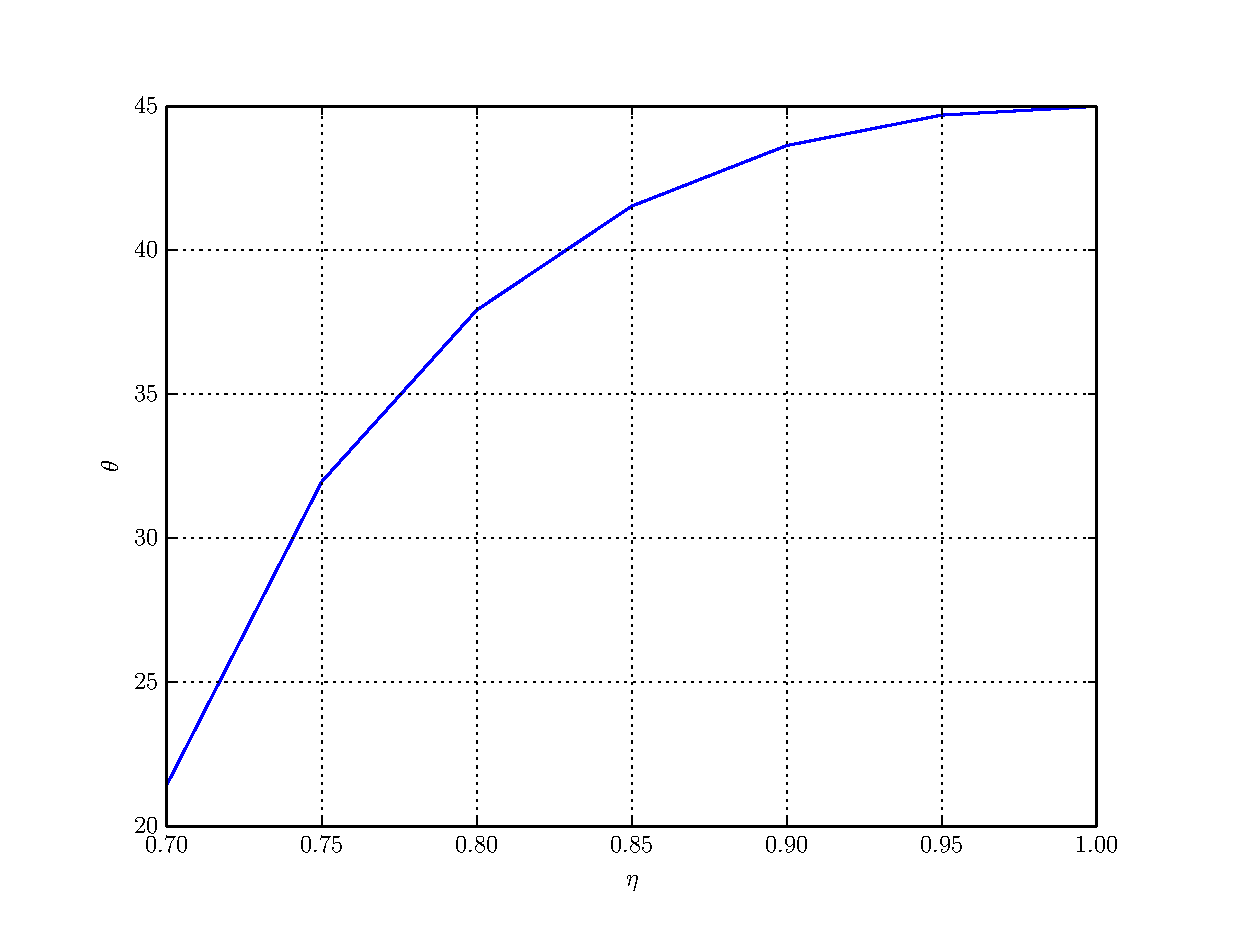
\includegraphics[scale=0.7]{theta.eps}
\caption{Optimized $\theta$ values for various detectors efficiency values}
\label{fig:theta_opt}
\end{figure}

\begin{figure}[h]
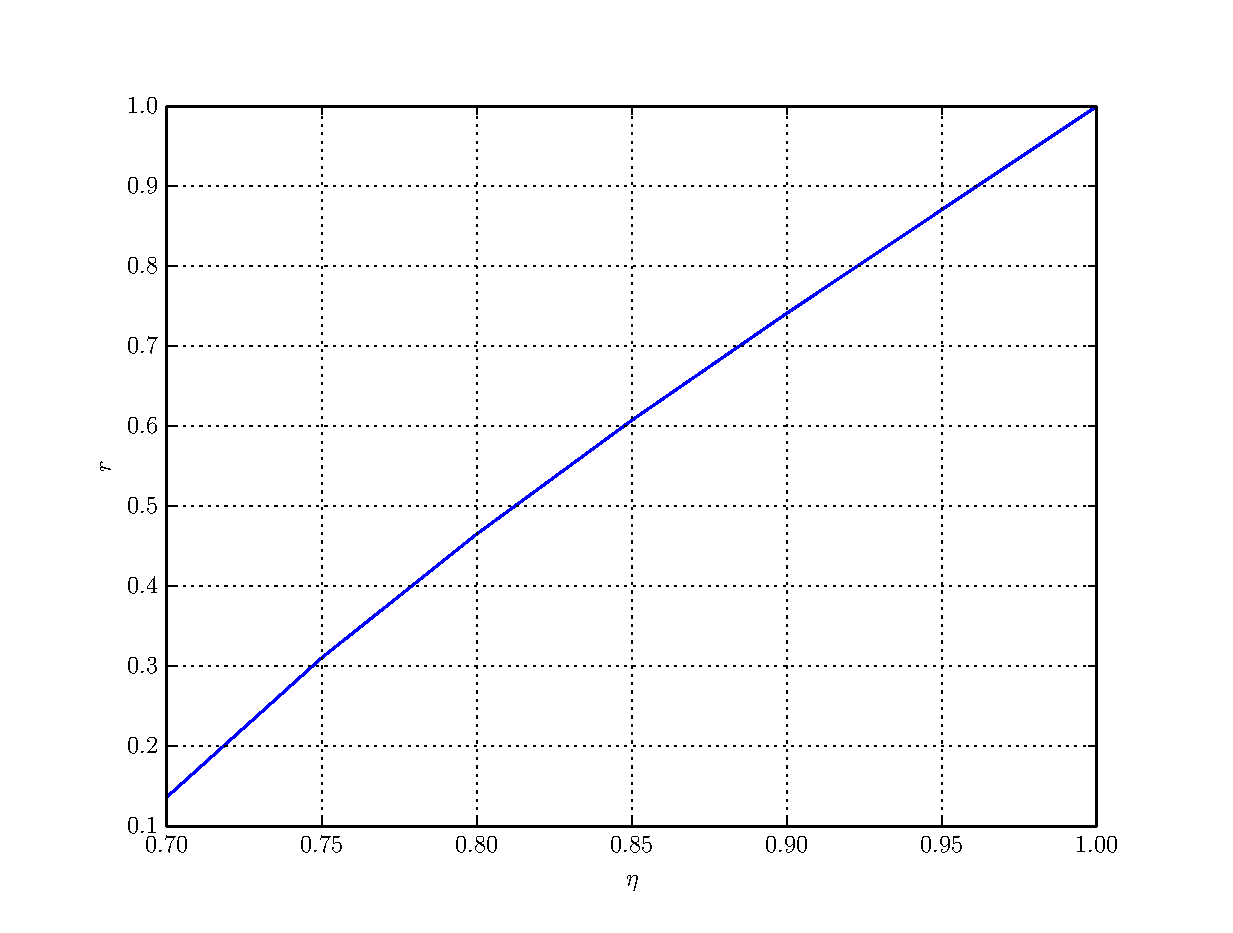
\includegraphics[scale=0.7]{r.eps}
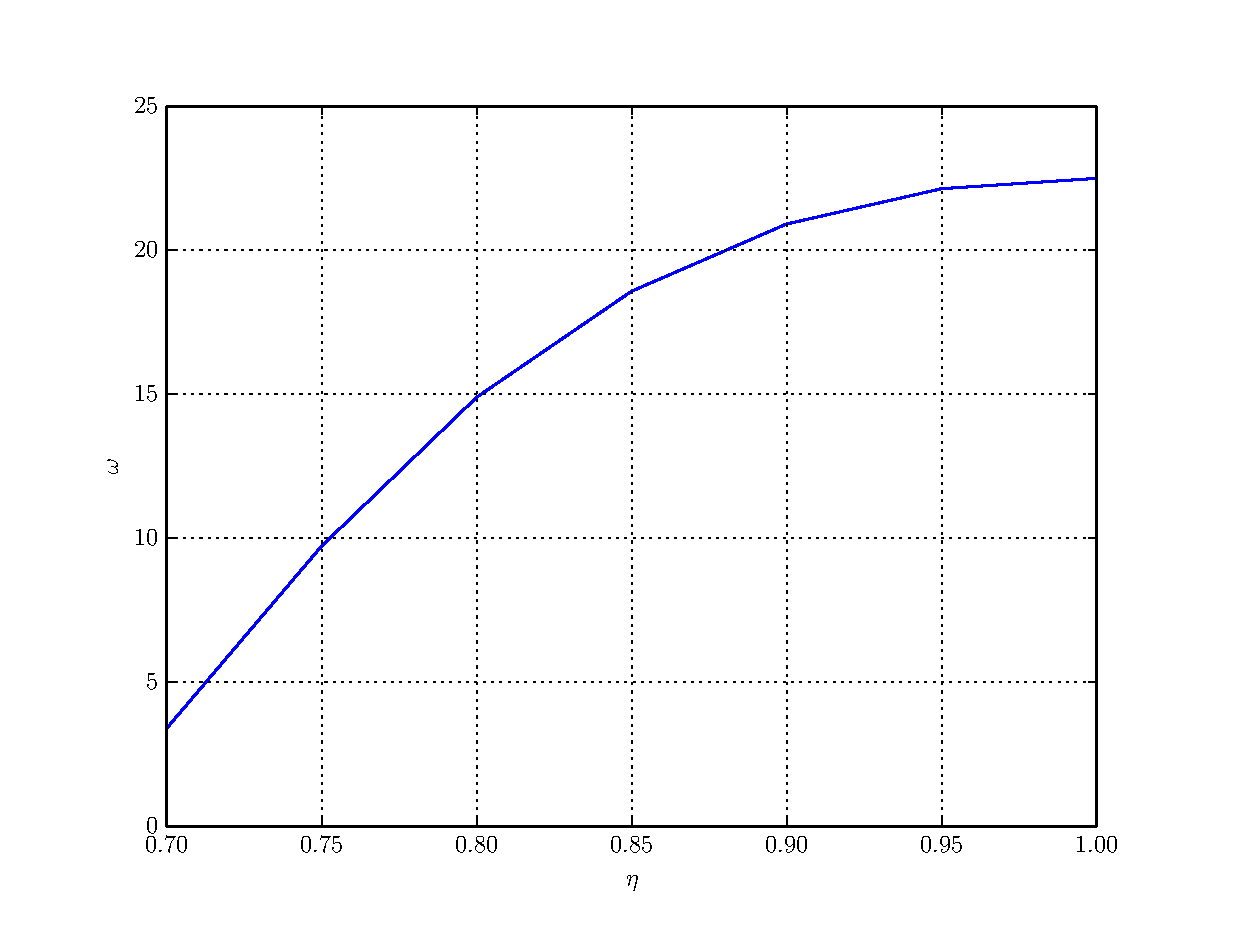
\includegraphics[scale=0.7]{omega.eps}
\caption{Optimized $r$ and $\omega$ values for various detectors efficiency values}
\label{fig:psi_opt}
\end{figure}

\begin{figure}[h]
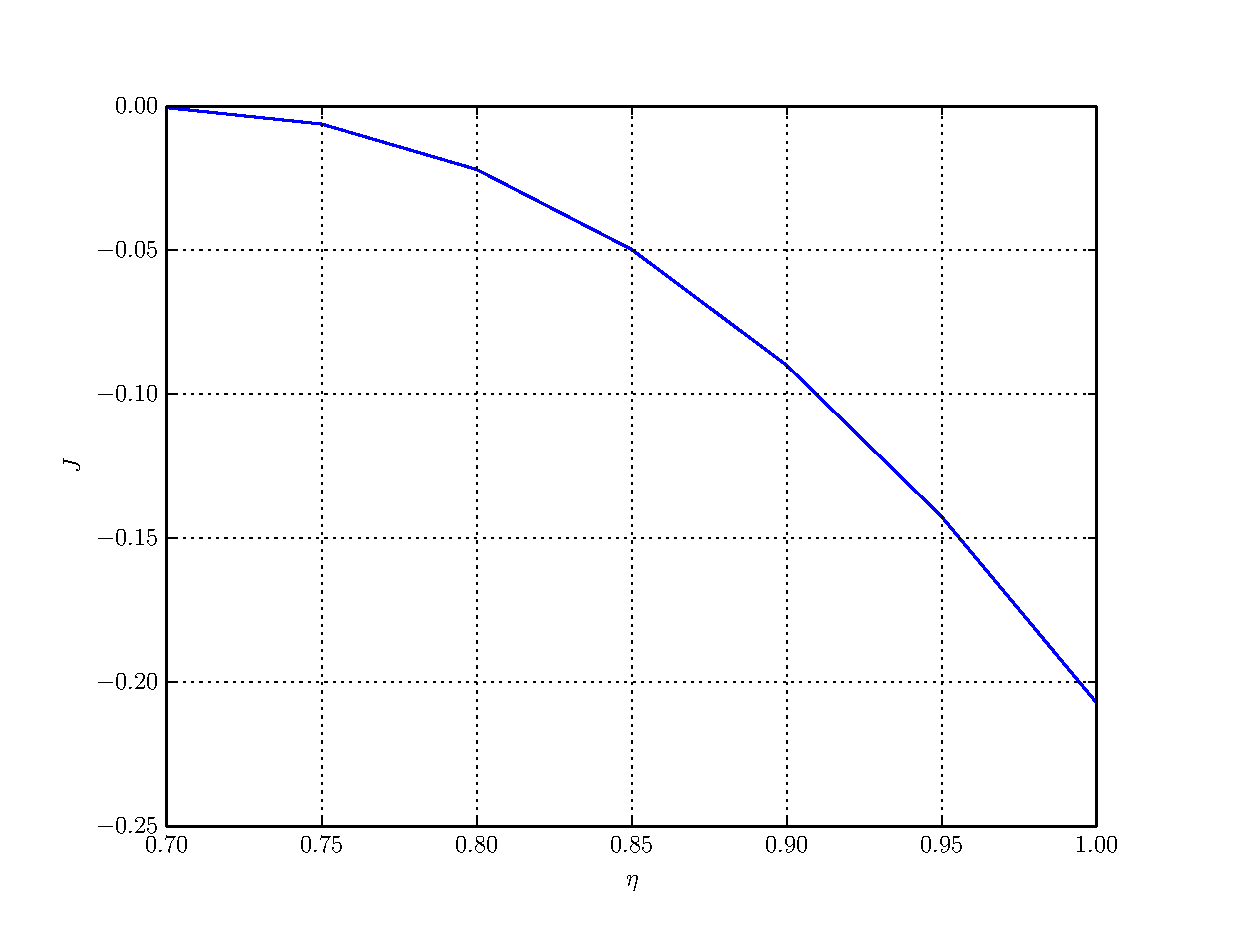
\includegraphics[scale=0.7]{J.eps}
\caption{Optimized $J_{\mathcal{B}}/N$ values for various detector efficiency values}
\label{fig:J_opt}
\end{figure}

At Fig. \ref{fig:theta_opt}, \ref{fig:psi_opt} relations between obtained parameters and efficiency 
are shown, at \ref{fig:J_opt} -- minimum function values obtained.

In real experiments detectors more often have different efficiency values, in this case 
formulas \eqref{eq:Eberhard_n_start}-\eqref{eq:Eberhard_n_finish} can be written as:
\begin{eqnarray*}
n_{oo}(\alpha_1, \beta_1) = N\frac{\eta_1\eta_2}{4}\psi^\dagger[I + \sigma(\alpha_1)][I + \tau(\beta_1)]\psi,\\
n_{oe}(\alpha_1, \beta_2) = N\frac{\eta_1\eta_2}{4}\psi^\dagger[I + \sigma(\alpha_1)][I - \tau(\beta_2)]\psi,\\
n_{ou}(\alpha_1, \beta_2) = N[\eta_1(1 - \eta_2)/2]\psi^\dagger[I + \sigma(\alpha_1)]\psi,\\
n_{eo}(\alpha_2, \beta_1) = N\frac{\eta_1\eta_2}{4}\psi^\dagger[I - \sigma(\alpha_2)][I + \tau(\beta_1)]\psi,\\
n_{uo}(\alpha_2, \beta_1) = N[\eta_2(1 - \eta_1)/2]\psi^\dagger[I + \tau(\beta_1)]\psi,\\
n_{oo}(\alpha_2, \beta_2) = N\frac{\eta_1\eta_2}{4}\psi^\dagger[I + \sigma(\alpha_2)][I + \tau(\beta_2)]\psi.
\end{eqnarray*}

\begin{figure}[h]
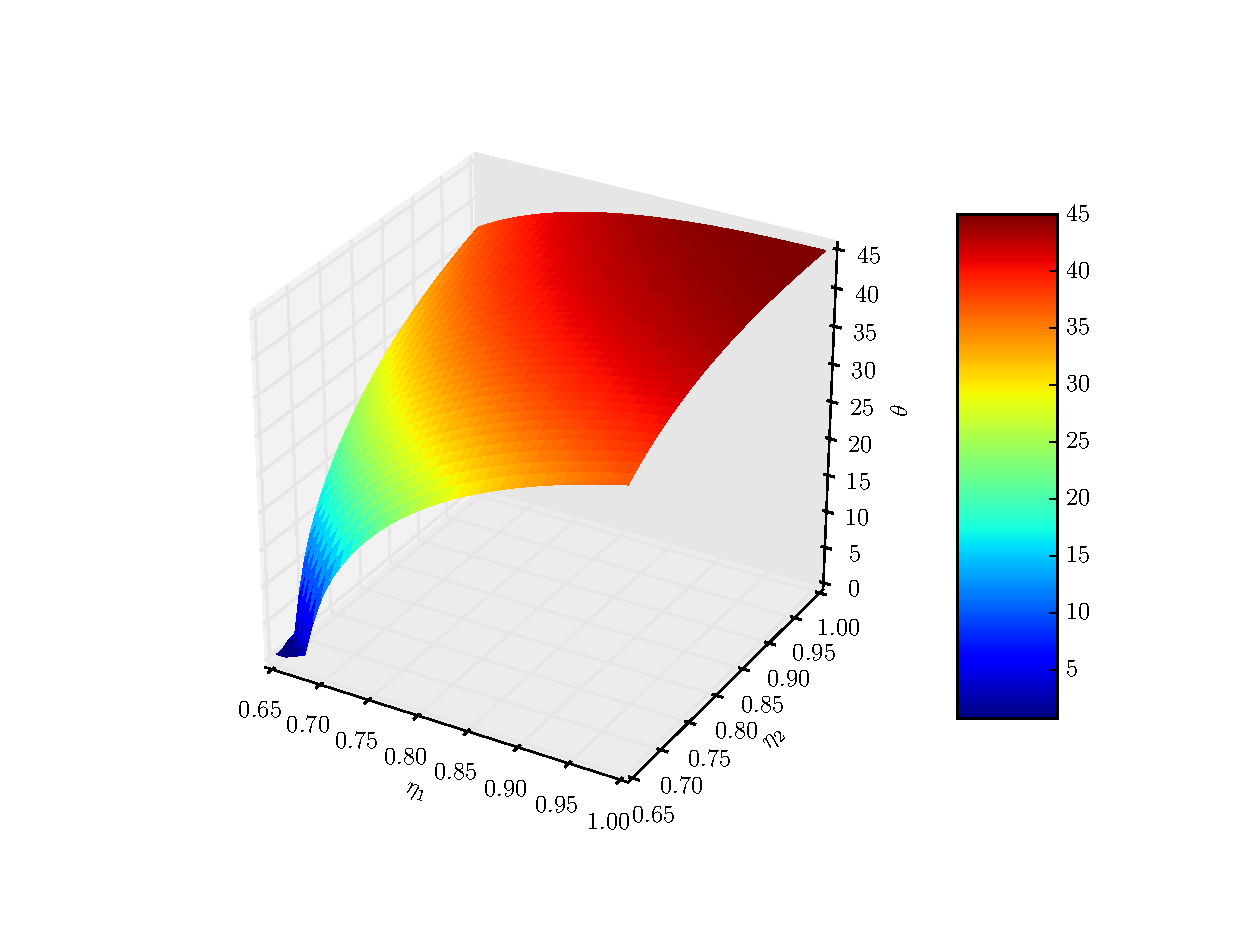
\includegraphics[scale=0.7]{theta3d.eps}
\caption{Optimized $\theta$ values for different detector efficiencies case}
\label{fig:theta_opt_3d}
\end{figure}

\begin{figure}[h]
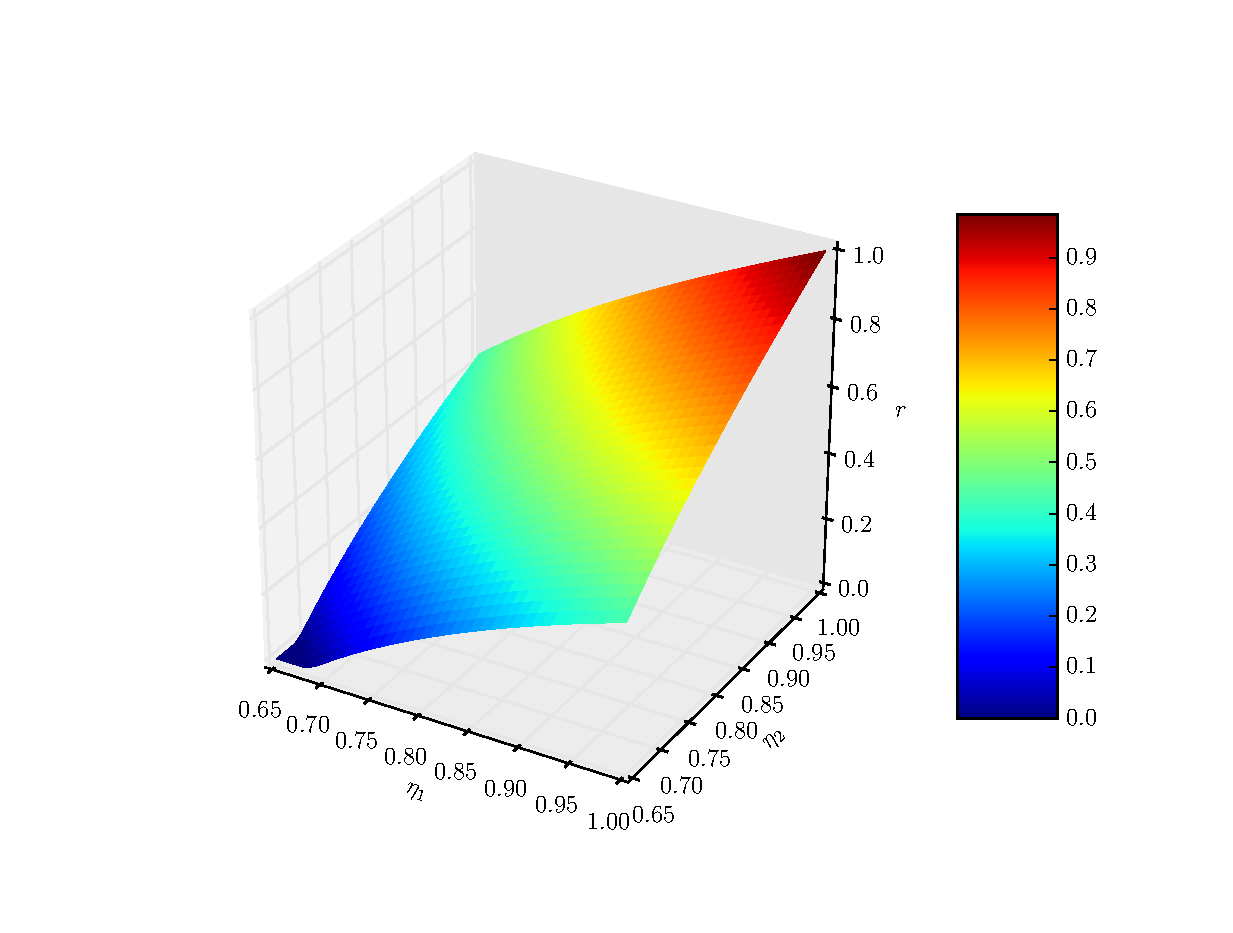
\includegraphics[scale=0.7]{r3d.eps}
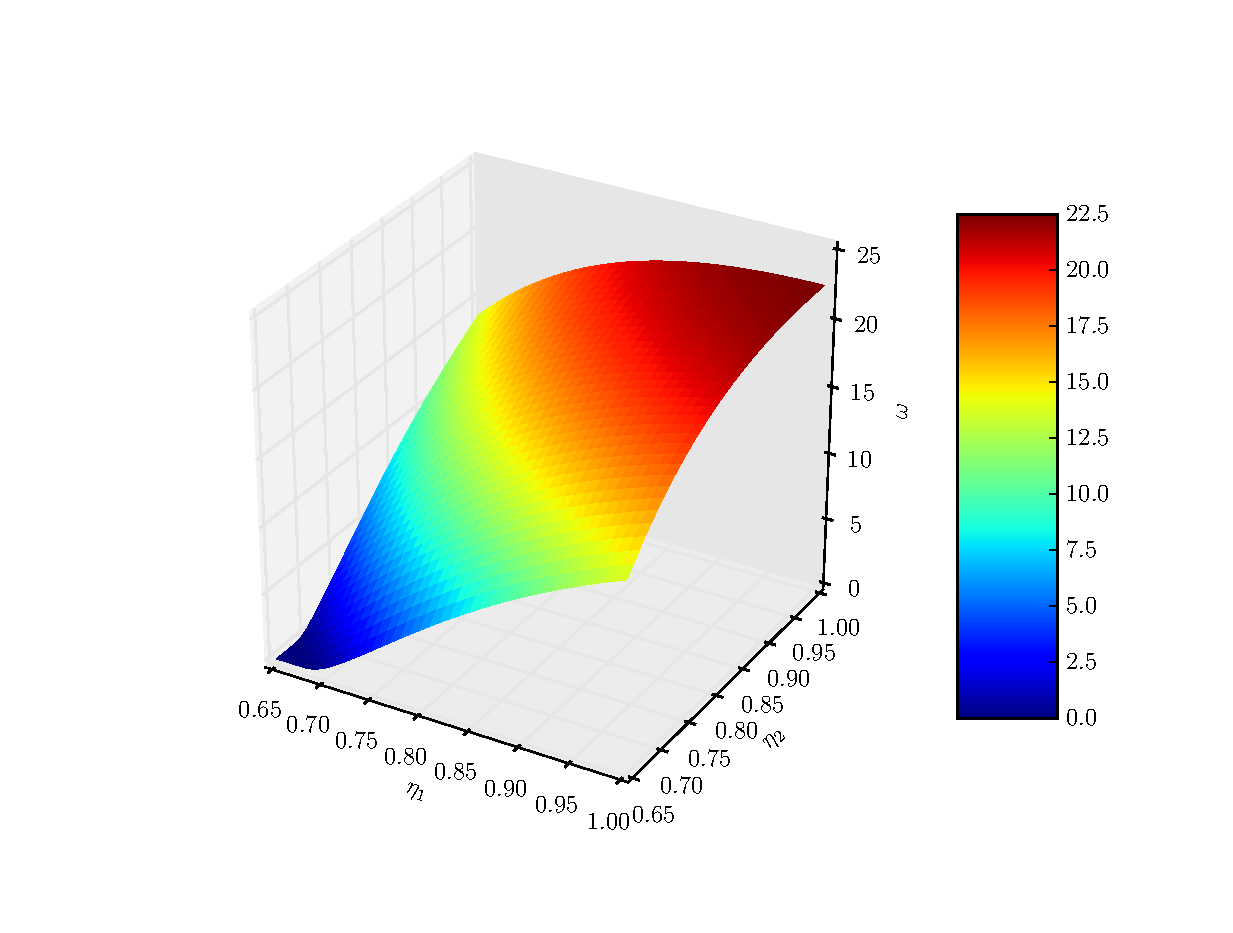
\includegraphics[scale=0.7]{omega3d.eps}
\caption{Optimized $r$ and $\omega$ values for different detector efficiencies case}
\label{fig:psi_opt_3d}
\end{figure}

\begin{figure}[t]
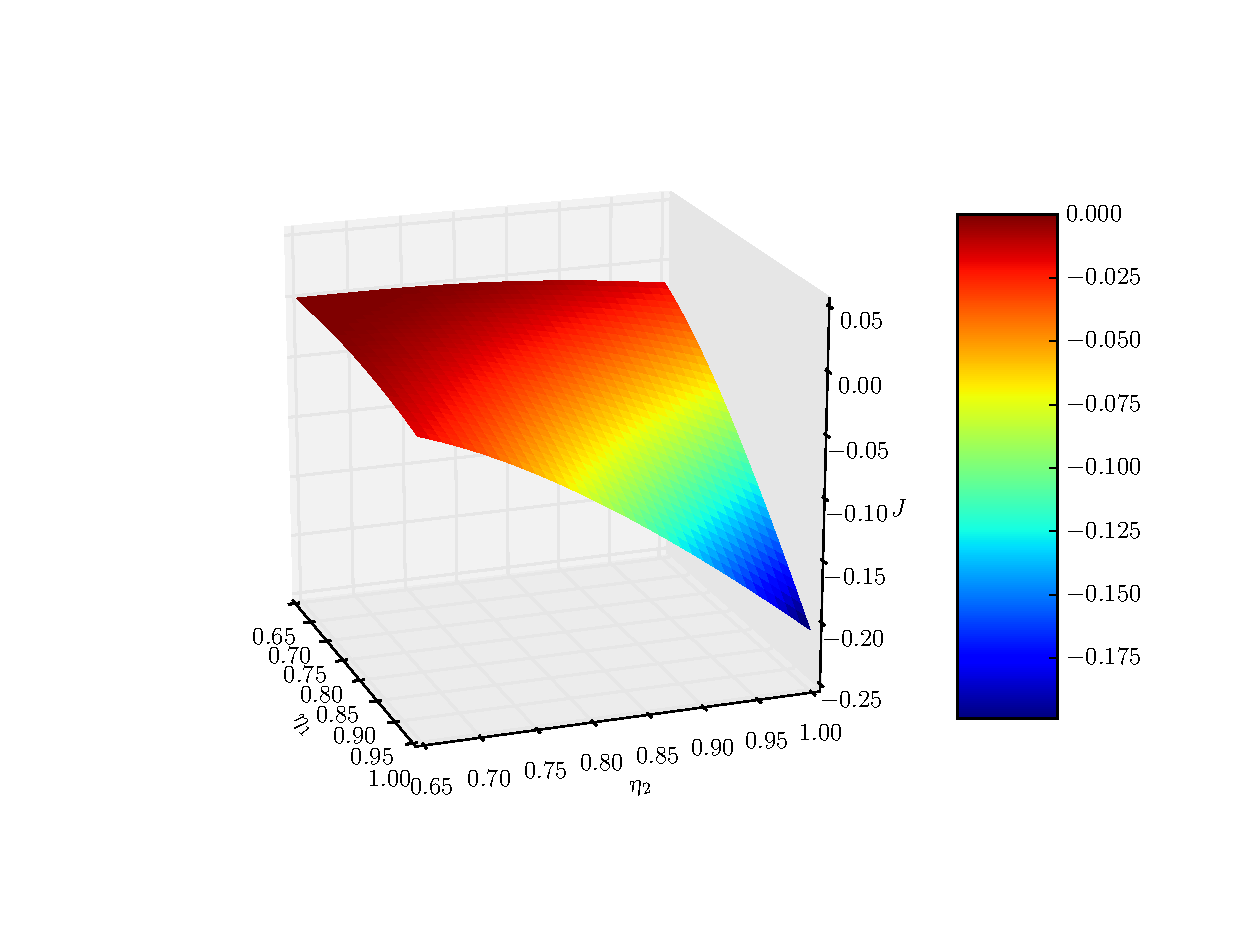
\includegraphics[scale=0.7]{J3d.eps}
\caption{Optimized $J_{\mathcal{B}}/N$ values for different detector efficiencies case}
\label{fig:J_opt_3d}
\end{figure}

At Fig.\ref{fig:theta_opt_3d} - \ref{fig:J_opt_3d} optimal parameters are shown, together with 
the minimised function for different detector efficiencies case.

\begingroup
\small

\begin{longtable}{|c|c|c|c|c|c|c|}
\hline
$\eta_1$ & $\eta_2$ & $r$ & $\omega,^\circ$ & $\theta,^\circ$ & $J_{\mathcal{B}}/N$ & $\zeta$
\\\hline
\endfirsthead

\hline
$\eta_1$ & $\eta_2$ & $r$ & $\omega,^\circ$ & $\theta,^\circ$ & $J_{\mathcal{B}}/N$ & $\zeta$
\\\hline
\endhead


\endfoot

\endlastfoot

\hline
0.65 & 0.65 & 9.73816e-05 & 5.32909e-05 & 0.609422 & 4.13366e-10 & --\\\hline
0.65 & 0.7 & 0.0325726 & 0.4367 & 10.3918 & -5.37452e-06 & 2.68726e-06\\\hline
0.65 & 0.75 & 0.122804 & 2.94407 & 20.3249 & -0.000327839 & 0.00016392\\\hline
0.65 & 0.8 & 0.199412 & 5.64399 & 25.8864 & -0.00152446 & 0.000762231\\\hline
0.65 & 0.85 & 0.266448 & 8.1196 & 29.7694 & -0.00385363 & 0.00192682\\\hline
0.65 & 0.9 & 0.326193 & 10.2951 & 32.6807 & -0.00737942 & 0.00368971\\\hline
0.65 & 0.95 & 0.380046 & 12.1725 & 34.9409 & -0.0120653 & 0.00603265\\\hline
0.65 & 1 & 0.42905 & 13.7822 & 36.7384 & -0.0178271 & 0.00891353\\\hline
0.7 & 0.65 & 0.0325721 & 0.436691 & 10.3917 & -5.37452e-06 & 2.68726e-06\\\hline
0.7 & 0.7 & 0.136389 & 3.40081 & 21.4266 & -0.000453562 & 0.000226781\\\hline
0.7 & 0.75 & 0.223629 & 6.53572 & 27.3754 & -0.00217282 & 0.00108641\\\hline
0.7 & 0.8 & 0.299639 & 9.33741 & 31.4432 & -0.00551773 & 0.00275887\\\hline
0.7 & 0.85 & 0.367155 & 11.7325 & 34.4284 & -0.0105412 & 0.00527059\\\hline
0.7 & 0.9 & 0.427895 & 13.7454 & 36.6985 & -0.0171516 & 0.0085758\\\hline
0.7 & 0.95 & 0.48304 & 15.4224 & 38.4617 & -0.0251977 & 0.0125989\\\hline
0.7 & 1 & 0.533433 & 16.8118 & 39.8493 & -0.034513 & 0.0172565\\\hline
0.75 & 0.65 & 0.122804 & 2.94407 & 20.3249 & -0.000327839 & 0.00016392\\\hline
0.75 & 0.7 & 0.223629 & 6.53572 & 27.3754 & -0.00217282 & 0.00108641\\\hline
0.75 & 0.75 & 0.310518 & 9.73143 & 31.9603 & -0.00615095 & 0.00307547\\\hline
0.75 & 0.8 & 0.387235 & 12.4151 & 35.2194 & -0.0123604 & 0.0061802\\\hline
0.75 & 0.85 & 0.455977 & 14.6188 & 37.6299 & -0.0206635 & 0.0103318\\\hline
0.75 & 0.9 & 0.518149 & 16.4057 & 39.45 & -0.0308332 & 0.0154166\\\hline
0.75 & 0.95 & 0.574864 & 17.8435 & 40.8423 & -0.0426257 & 0.0213128\\\hline
0.75 & 1 & 0.626962 & 18.9919 & 41.9138 & -0.0558135 & 0.0279068\\\hline
0.8 & 0.65 & 0.199412 & 5.64399 & 25.8864 & -0.00152446 & 0.000762231\\\hline
0.8 & 0.7 & 0.299639 & 9.33741 & 31.4432 & -0.00551773 & 0.00275887\\\hline
0.8 & 0.75 & 0.387235 & 12.4151 & 35.2194 & -0.0123604 & 0.0061802\\\hline
0.8 & 0.8 & 0.465228 & 14.8979 & 37.9215 & -0.02191 & 0.010955\\\hline
0.8 & 0.85 & 0.535462 & 16.8648 & 39.9011 & -0.0338613 & 0.0169307\\\hline
0.8 & 0.9 & 0.59933 & 18.4036 & 41.3692 & -0.0478775 & 0.0239387\\\hline
0.8 & 0.95 & 0.657889 & 19.5935 & 42.4623 & -0.063646 & 0.031823\\\hline
0.8 & 1 & 0.712001 & 20.5014 & 43.274 & -0.0808982 & 0.0404491\\\hline
0.85 & 0.65 & 0.266448 & 8.1196 & 29.7694 & -0.00385363 & 0.00192682\\\hline
0.85 & 0.7 & 0.367155 & 11.7325 & 34.4284 & -0.0105412 & 0.00527059\\\hline
0.85 & 0.75 & 0.455977 & 14.6188 & 37.6299 & -0.0206635 & 0.0103318\\\hline
0.85 & 0.8 & 0.535462 & 16.8648 & 39.9011 & -0.0338613 & 0.0169307\\\hline
0.85 & 0.85 & 0.607424 & 18.5808 & 41.5341 & -0.0496902 & 0.0248451\\\hline
0.85 & 0.9 & 0.673214 & 19.8694 & 42.7109 & -0.0677295 & 0.0338647\\\hline
0.85 & 0.95 & 0.733924 & 20.817 & 43.552 & -0.087619 & 0.0438095\\\hline
0.85 & 1 & 0.790464 & 21.4958 & 44.1427 & -0.109064 & 0.0545318\\\hline
0.9 & 0.65 & 0.326193 & 10.2951 & 32.6807 & -0.00737942 & 0.00368971\\\hline
0.9 & 0.7 & 0.427895 & 13.7454 & 36.6985 & -0.0171516 & 0.0085758\\\hline
0.9 & 0.75 & 0.518149 & 16.4057 & 39.45 & -0.0308332 & 0.0154166\\\hline
0.9 & 0.8 & 0.59933 & 18.4036 & 41.3692 & -0.0478775 & 0.0239387\\\hline
0.9 & 0.85 & 0.673214 & 19.8694 & 42.7109 & -0.0677295 & 0.0338647\\\hline
0.9 & 0.9 & 0.741202 & 20.9153 & 43.6381 & -0.0899078 & 0.0449539\\\hline
0.9 & 0.95 & 0.804477 & 21.6349 & 44.2627 & -0.11402 & 0.0570101\\\hline
0.9 & 1 & 0.863896 & 22.1002 & 44.661 & -0.139755 & 0.0698776\\\hline
0.95 & 0.65 & 0.380046 & 12.1725 & 34.9409 & -0.0120653 & 0.00603265\\\hline
0.95 & 0.7 & 0.48304 & 15.4224 & 38.4617 & -0.0251977 & 0.0125989\\\hline
0.95 & 0.75 & 0.574864 & 17.8435 & 40.8423 & -0.0426257 & 0.0213128\\\hline
0.95 & 0.8 & 0.657889 & 19.5935 & 42.4623 & -0.063646 & 0.031823\\\hline
0.95 & 0.85 & 0.733924 & 20.817 & 43.552 & -0.087619 & 0.0438095\\\hline
0.95 & 0.9 & 0.804477 & 21.6349 & 44.2627 & -0.11402 & 0.0570101\\\hline
0.95 & 0.95 & 0.87067 & 22.141 & 44.6958 & -0.142436 & 0.0712182\\\hline
0.95 & 1 & 0.933431 & 22.4101 & 44.924 & -0.172546 & 0.086273\\\hline
1 & 0.65 & 0.42905 & 13.7822 & 36.7384 & -0.0178271 & 0.00891353\\\hline
1 & 0.7 & 0.533433 & 16.8118 & 39.8493 & -0.034513 & 0.0172565\\\hline
1 & 0.75 & 0.626962 & 18.9919 & 41.9138 & -0.0558135 & 0.0279068\\\hline
1 & 0.8 & 0.712001 & 20.5014 & 43.274 & -0.0808982 & 0.0404491\\\hline
1 & 0.85 & 0.790464 & 21.4958 & 44.1427 & -0.109064 & 0.0545318\\\hline
1 & 0.9 & 0.863896 & 22.1002 & 44.661 & -0.139755 & 0.0698776\\\hline
1 & 0.95 & 0.933431 & 22.4101 & 44.924 & -0.172546 & 0.086273\\\hline
1 & 1 & 0.999997 & 22.5 & 45 & -0.207107 & 0.103553\\\hline
\caption{Optimal parameters values for different detector efficiencies case}
\label{tab:different_etas}
\end{longtable}

\endgroup

Parameters values obtained during optimization process along with maximal allowable noise level 
are shown in Table~\ref{tab:different_etas}. The bigger each value of efficiency separately, the more 
strongly inequality can be violated. Minimal efficiency values for which violation is possible are close 
to  $\eta_1 = \eta_2 = 0.67$ value, matching Eberhard results.

%\clearpage

Generally for every state $\psi$ minimizing expectancy value the following corollary holds.

\begin{theorem}
Quantum state $\psi$ minimizing target function $J$ is an eigenvector of matrix $\mathcal{B}$ and 
transforms dispersion to zero.
\end{theorem}
\begin{proof}
By Courant–Fischer theorem $\lambda_1 \leq \langle\mathcal{B}\psi, \psi\rangle \leq \lambda_n$, where $\lambda_1, \ldots \lambda_n$ -- eigenvalues, sorted in ascending order. Minimum 
$J_\mathcal{B} = \langle\mathcal{B}\psi, \psi\rangle = \lambda_1$ is reached if $\psi = \psi_1$ is an 
eigenvector.

For the dispersion value in this case we have:
\[\sigma^2 = \langle B^2\rangle - \langle B\rangle^2 = \psi^\dagger B^2 \psi - \lambda_1^2 = \psi^\dagger B \lambda_1  \psi - \lambda_1^2 = 0.
\]
\end{proof}

It means that the obtained states are optimal not only from mathematical expectancy point of view 
for various combinations amount of polarization measurements, but also from 
possible scatter of measurement results expressed in terms of dispersion point of view.

\section{Parameters optimization for Zeilinger model}
In article \cite{Zeilinger} Eberhard inequality check applied to the real experiment is considered. 
During experiment conditions $n_{ou}, n_{uo}$ values were found by the following formulas:
\[
n_{ou}(\alpha_1, \beta_2) = S_o^A(\alpha_1) - n_{oo}(\alpha_1, \beta_2) - n_{oe}(\alpha_1, \beta_2),
\]
\[
n_{uo}(\alpha_2, \beta_1) = S_o^B(\beta_1) - n_{oo}(\alpha_2, \beta_1) - n_{eo}(\alpha_2, \beta_1),
\]
where $S_o^A, S_o^B$ -- the amount of clicks in the usual beam for first and second system 
correspondingly.

In this case Eberhard inequality takes form:
\begin{equation}
J = -n_{oo}(\alpha_1, \beta_1) + S_o^A(\alpha_1) - n_{oo}(\alpha_1, \beta_2) + S_o^B(\beta_1) - n_{oo}(\alpha_2, \beta_1) + n_{oo}(\alpha_2, \beta_2) \geq 0
\label{eq:Zeilinger_J}
\end{equation}

Consider density operator as a quantum state of the system:
\[
\rho = \frac{1}{\sqrt{1+r^2}}
\begin{vmatrix}
0 & 0 & 0 & 0\\
0 & 1 & Vr & 0\\
0 & Vr & r^2 & 0\\
0 & 0 & 0 & 0
\end{vmatrix},
\]
where $0 \leq r \leq 1$ и $0 \leq V \leq 1$.
In this case predictions of quantum mechanics for values included to inequality become:
\begin{eqnarray*}
\tilde{S}_o^A(\alpha_i) = \eta_1 N \Tr[\rho(\hat{P}_A(\alpha_i) \otimes I)]\\
\tilde{S}_o^B(\beta_i) = \eta_1 N \Tr[\rho(I \otimes \hat{P}_B(\beta_i))]\\
\tilde{n}_{oo}(\alpha_i, \beta_i) = \eta_1\eta_2 N \Tr[\rho(\hat{P}_A(\alpha_i) \otimes \hat{P}_B(\beta_i))],
\end{eqnarray*}
where $\hat{P}_A, \hat{P}_B$ -- projection operators on usual beam direction for the first and second prism:
\[
\hat{P}(\gamma) = 
\begin{pmatrix}
\cos^2\gamma & \cos\gamma\sin\gamma\\
\cos\gamma\sin\gamma & \sin^2\gamma
\end{pmatrix}.
\]

With regard to false clicks during time $T$ $S_o^A, S_o^B$ values take form:
\[
S_o^A(\alpha_i) = \tilde{S}_o^A(\alpha_i) + \zeta T,
\]
\[
S_o^B(\beta_i) = \tilde{S}_o^B(\beta_i) + \zeta T.
\]

Besides noise Zeilinger model also considers inconsistencies in time when pairs from different 
launches are detected as a conjugate events. Let us introduce temporary window value $\tau_c$, within 
which conjugate events must be detected. In this case $n_{oo}(\alpha_i, \beta_i)$ can be found using 
the following formulas:
\[
n_{oo}(\alpha_i, \beta_i) = \tilde{n}_{oo}(\alpha_i, \beta_i) + n_{oo}^{acc}(\alpha_i, \beta_i),
\]
\[
n_{oo}^{acc}(\alpha_i, \beta_i) = S_o^A(\alpha_i)S_o^B(\beta_i)\frac{\tau_c}{T}\left(1 - \frac{\tilde{n}_{oo}(\alpha_i, \beta_i)}{S_o^A(\alpha_i)}\right) \left( 1 - \frac{\tilde{n}_{oo}(\alpha_i, \beta_i)}{S_o^B(\beta_i)}\right).
\]

For this model an optimization for $J$ \eqref{eq:Zeilinger_J} was done, during which angle values 
minimising target function were found for selected values of experimental parameters 
($\eta_1, \eta_2, r, V, T, \tau_c, N, \zeta$).

\begin{table}
\begin{tabular}{|c|c|c|c|c|c|}
\hline 
 & $\alpha_1, ^\circ$ & $\alpha_2, ^\circ$ & $\beta_1, ^\circ$ & $\beta_2, ^\circ$ & $J$ \\ 
\hline 
Results from the article & 85.6 & 118.0 & -5.4 & 25.9 & -120191 \\ 
\hline 
Results of optimization & 85.0 & 115.1 & -4.0 & 27.4 & -126060 \\ 
\hline 
\end{tabular}
\caption{Optimal parameters comparison with ones from Zeilinger article \cite{Zeilinger}}
\label{tab:Zeilinger_parameters}
\end{table}

Optimization results are shown in Table~\ref{tab:Zeilinger_parameters}. According to obtained values, 
optimal angle values for prism installation differ from given in \cite{Zeilinger} and let inequality to be 
violated stronger.

\section{Inequality parameters search in the case of errors when setting angle values}
Generally quantum operator $A$ can be represented using spectral decomposition as 
$A = \int_{-\infty}^{+\infty}\lambda dE_\lambda$. Then it's mathematical expectancy value for $\psi$ 
state can be expressed as:
\[
\overline{A}_\psi = \int_{-\infty}^{+\infty}\lambda dp_\psi (\lambda),
\]
where $dp_\psi (\lambda) = d\langle E_\lambda\psi, \psi\rangle$ -- probability distribution for the 
corresponding spectral expansion and quantum state. Therefore for fixed $\psi$ quantum observable 
can be regarded as classical random variable with probabilities distribution
$p_\psi (O) = \int_O d\langle E_\lambda\psi, \psi\rangle, O\in \mathbb{R}$.

Consider the following problem. Let observable $A$ to depend on some classical random variable 
$\omega: A = A(\omega)$ corresponding to the case when angle values for the prisms positions 
cannot be exactly set during experiments. In this case spectral decomposition 
$A(\omega) = \int_{-\infty}^{+\infty}\lambda dE_\lambda(\omega)$ and density distribution function 
$dp_\psi (\lambda|\omega) = d\langle E_\lambda(\omega)\psi, \psi\rangle$ also depends on 
this random variable. For every fixed $\omega$ also 
$\int_{-\infty}^{+\infty}dp_\psi (\lambda|\omega) = 1$ condition holds.

Let random variable $\omega$ be described using probability space $(\Omega, \mathcal{F}, P)$, 
where $\Omega$ -- set of elementary events, $\mathcal{F}$ - $\sigma$-algebra of events and 
$P$ is the probability measure. Mathematical expectancy value of $A(\omega)$ becomes:
\[
\overline{A}_\psi(\omega) = \int_\Omega\left[\int_{-\infty}^{+\infty}\lambda dp_\psi (\lambda|\omega)\right] dP(\omega) = \int_\Omega\langle A(\omega)\psi, \psi\rangle dP(\omega) = \mathbf{\tilde{E}}[ \langle A(\omega)\psi, \psi\rangle],
\]
where $\mathbf{\tilde{E}}[\cdot]$ -- classical mathematical expectancy.

Similarly we obtained an expression for dispersion $A(\omega)$:
\[
\sigma^2(A) = \mathbf{\tilde{E}}[ \langle A^2(\omega)\psi, \psi\rangle - \langle A(\omega)\psi, \psi\rangle^2].
\]

Consider real value of $\theta$ angles' difference to be uniformly distributed at the sector around 
the desired value in the experiment. In this case $\theta' = \theta + \xi$, where $\xi$ -- random variable, 
uniformly distributed at $[-\delta; \delta]$ sector, $\delta > 0$ -- scatter parameter. Then
\[
J_\mathcal{B} = \frac{1}{2\delta}\int_{-\delta}^\delta \langle \mathcal{B}(r, \omega, \theta + x)\psi, \psi \rangle dx
\] and
\[
\sigma^2 = \frac{1}{2\delta}\int_{-\delta}^\delta (\langle \mathcal{B}^2(r, \omega, \theta + x)\psi, \psi \rangle - \langle \mathcal{B}(r, \omega, \theta + x)\psi, \psi \rangle^2) dx.
\]

Consider also target function that takes into account relative scatter of values obtained, expressed with 
$J / \sigma$ variance coefficient. It enables us to obtain parameters for which  relative value will be minimal 
with some scatter of experimental data.

\begin{figure}[h]
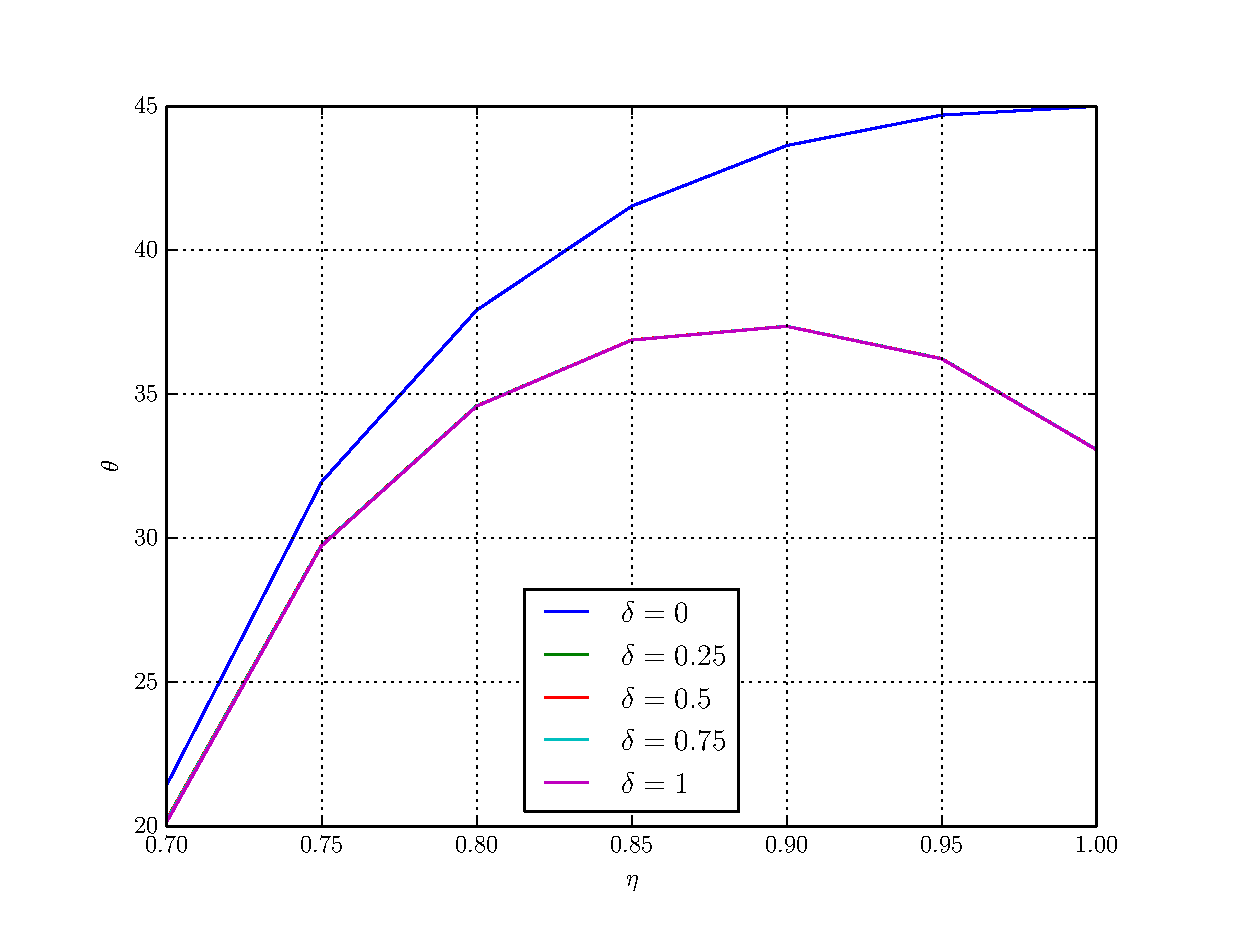
\includegraphics[scale=0.7]{theta_ang.eps}
\caption{Optimized values for $\theta$ for various $\delta$ values case of $\theta' = \theta + \xi$}
\label{fig:theta_ang}
\end{figure}

\begin{figure}[h]
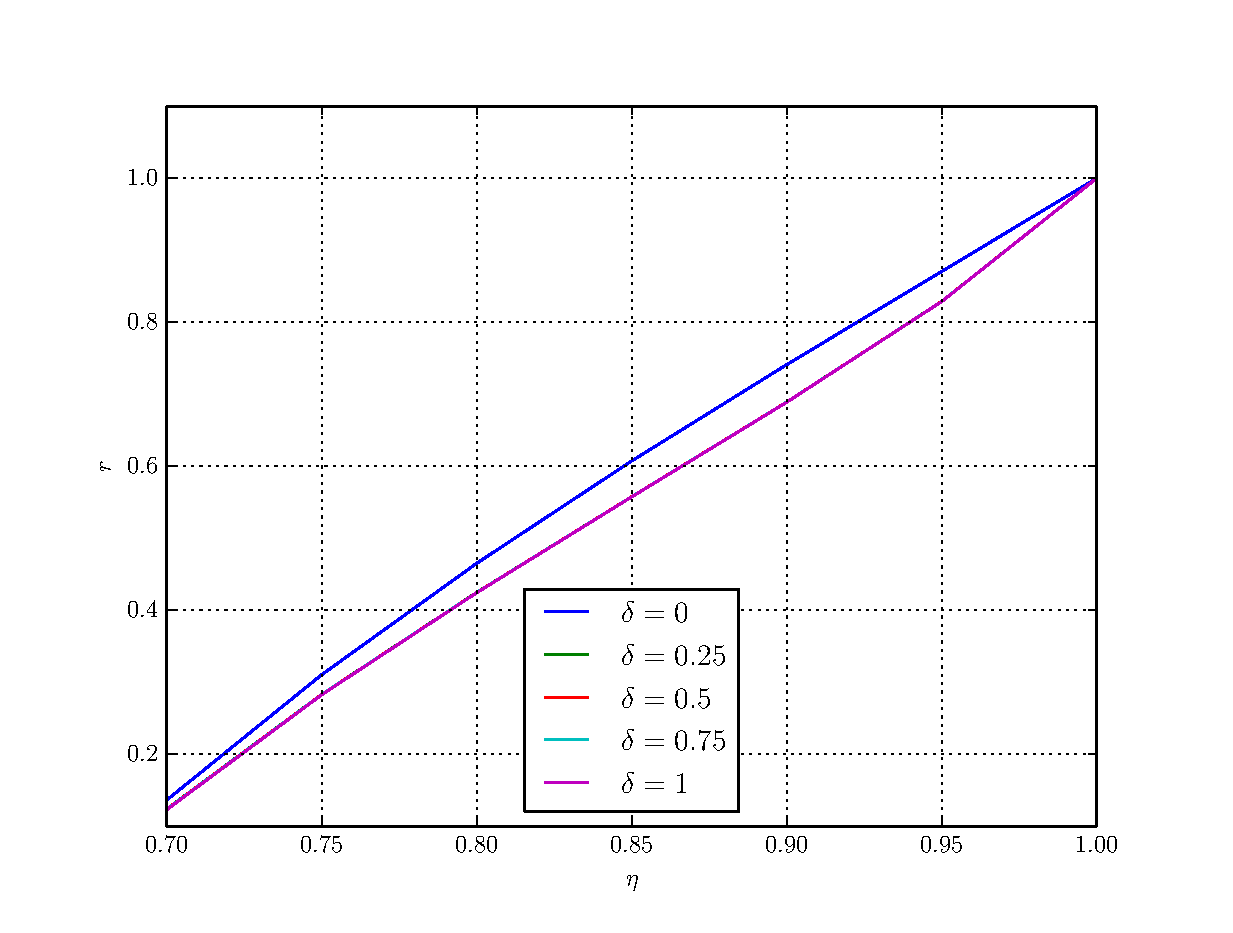
\includegraphics[scale=0.7]{r_ang.eps}
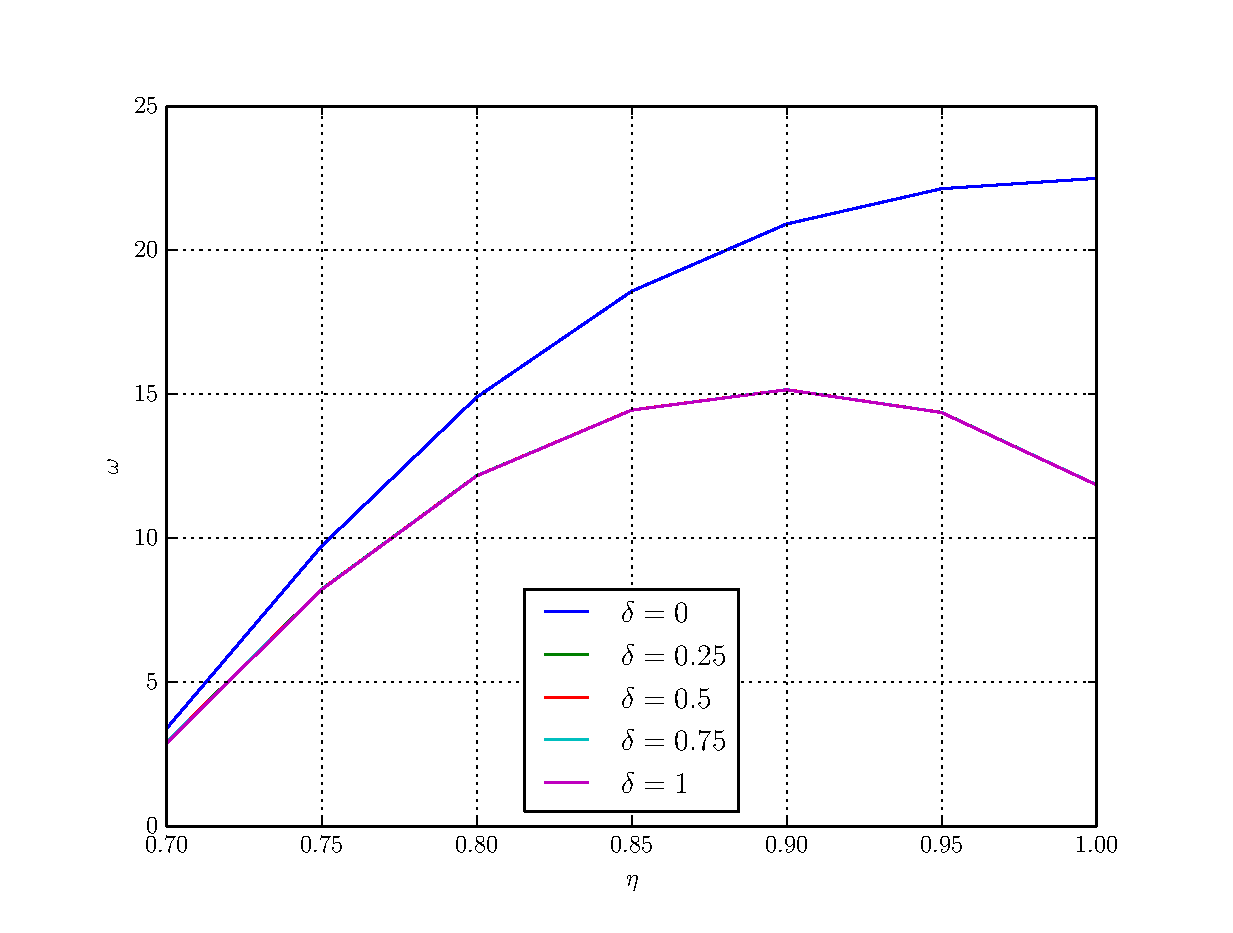
\includegraphics[scale=0.7]{omega_ang.eps}
\caption{Optimized values for $r$ and $\omega$ for various $\delta$ values case of $\theta' = \theta + \xi$}
\label{fig:psi_ang}
\end{figure}

\begin{figure}[t]
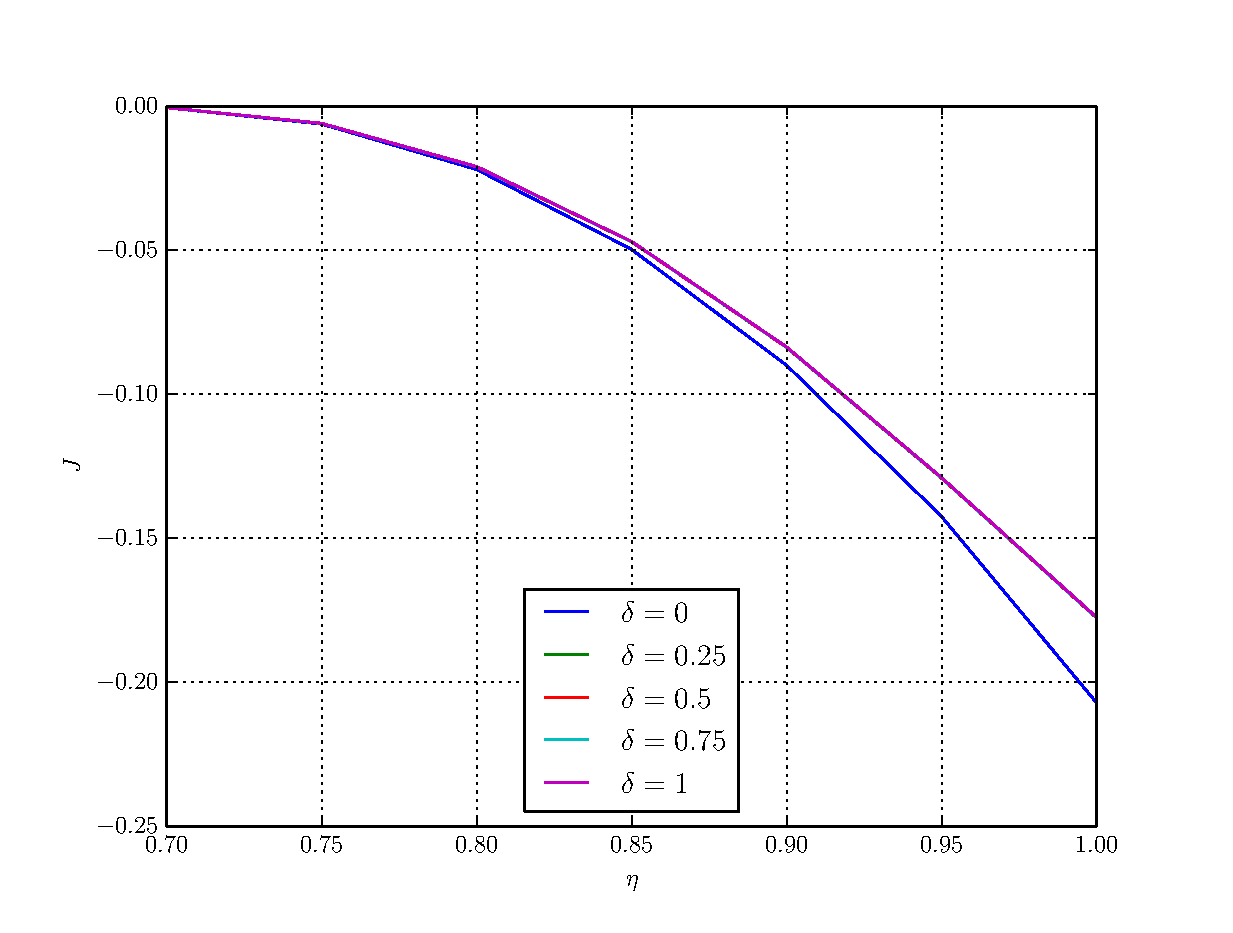
\includegraphics[scale=0.7]{J_ang.eps}
\caption{Optimized values for $J_{\mathcal{B}}/N$ for various $\delta$ values case of $\theta' = \theta + \xi$}
\label{fig:J_ang}
\end{figure}

%%%%%%%%%%%%%%%%%%%%%%%%%%%%%%%%%%%%%%%%%%%%%%%%%

\begingroup
\small

\begin{longtable}{|c|c|c|c|c|c|c|c|c|}
\hline
$\eta$ & $\delta,^\circ$ & $r$ & $\omega,^\circ$ & $\theta,^\circ$ & $J$ & $J_{\delta}$ & $\sigma_{\delta}$ & $K = J_{\delta}/\sigma_{\delta}$
\endfirsthead

\hline
$\eta$ & $\delta,^\circ$ & $r$ & $\omega,^\circ$ & $\theta,^\circ$ & $J$ & $J_{\delta}$ & $\sigma_{\delta}$ & $K = J_{\delta}/\sigma_{\delta}$\\
\hline
\endhead

\hline
\endfoot

\endlastfoot

\hline
\multirow{3}{*}{0.7} & \multirow{3}{*}{0.25} & 0.13639 & 3.4008 & 21.427 & -0.00045356 & -0.00045189 & 0.00087956 & -0.51377\\\cline{3-9}
 &  & 0.13629 & 3.3972 & 21.418 & -0.00045356 & -0.00045189 & 0.00087922 & -0.51397\\\cline{3-9}
 &  & 0.12395 & 2.9245 & 20.237 & -0.00044085 & -0.00043936 & 0.00083444 & -0.52653\\\hline
\multirow{3}{*}{0.7} & \multirow{3}{*}{0.5} & 0.13639 & 3.4008 & 21.427 & -0.00045356 & -0.00044688 & 0.0017591 & -0.25404\\\cline{3-9}
 &  & 0.1361 & 3.3903 & 21.397 & -0.00045355 & -0.00044689 & 0.0017569 & -0.25437\\\cline{3-9}
 &  & 0.12378 & 2.9192 & 20.221 & -0.00044051 & -0.00043455 & 0.0016676 & -0.26059\\\hline
\multirow{3}{*}{0.7} & \multirow{3}{*}{0.75} & 0.13639 & 3.4008 & 21.427 & -0.00045356 & -0.00043854 & 0.0026387 & -0.1662\\\cline{3-9}
 &  & 0.13566 & 3.3739 & 21.357 & -0.00045351 & -0.00043858 & 0.0026307 & -0.16672\\\cline{3-9}
 &  & 0.1235 & 2.91 & 20.193 & -0.00043993 & -0.00042657 & 0.0024981 & -0.17076\\\hline
\multirow{3}{*}{0.7} & \multirow{3}{*}{1.0} & 0.13639 & 3.4008 & 21.427 & -0.00045356 & -0.00042685 & 0.0035182 & -0.12132\\\cline{3-9}
 &  & 0.13513 & 3.3554 & 21.305 & -0.00045341 & -0.000427 & 0.0034994 & -0.12202\\\cline{3-9}
 &  & 0.12306 & 2.8955 & 20.149 & -0.000439 & -0.00041536 & 0.0033239 & -0.12496\\\hline
\multirow{3}{*}{0.75} & \multirow{3}{*}{0.25} & 0.31052 & 9.7314 & 31.96 & -0.0061509 & -0.0061468 & 0.0014539 & -4.2279\\\cline{3-9}
 &  & 0.31047 & 9.729 & 31.956 & -0.0061509 & -0.0061468 & 0.0014537 & -4.2284\\\cline{3-9}
 &  & 0.28314 & 8.2348 & 29.774 & -0.0059469 & -0.0059433 & 0.0013654 & -4.3528\\\hline
\multirow{3}{*}{0.75} & \multirow{3}{*}{0.5} & 0.31052 & 9.7314 & 31.96 & -0.0061509 & -0.0061346 & 0.0029077 & -2.1098\\\cline{3-9}
 &  & 0.31037 & 9.7245 & 31.95 & -0.0061509 & -0.0061346 & 0.0029068 & -2.1104\\\cline{3-9}
 &  & 0.28301 & 8.2297 & 29.765 & -0.0059453 & -0.0059309 & 0.00273 & -2.1725\\\hline
\multirow{3}{*}{0.75} & \multirow{3}{*}{0.75} & 0.31052 & 9.7314 & 31.96 & -0.0061509 & -0.0061141 & 0.0043614 & -1.4019\\\cline{3-9}
 &  & 0.31024 & 9.7187 & 31.939 & -0.0061509 & -0.0061141 & 0.0043587 & -1.4027\\\cline{3-9}
 &  & 0.28288 & 8.2252 & 29.756 & -0.0059437 & -0.0059113 & 0.0040937 & -1.444\\\hline
\multirow{3}{*}{0.75} & \multirow{3}{*}{1.0} & 0.31052 & 9.7314 & 31.96 & -0.0061509 & -0.0060854 & 0.0058149 & -1.0465\\\cline{3-9}
 &  & 0.30998 & 9.7066 & 31.92 & -0.0061509 & -0.0060854 & 0.005808 & -1.0478\\\cline{3-9}
 &  & 0.28269 & 8.219 & 29.743 & -0.0059414 & -0.0058839 & 0.0054558 & -1.0785\\\hline
\multirow{3}{*}{0.8} & \multirow{3}{*}{0.25} & 0.46523 & 14.898 & 37.921 & -0.02191 & -0.021904 & 0.0019372 & -11.307\\\cline{3-9}
 &  & 0.46523 & 14.898 & 37.921 & -0.02191 & -0.021904 & 0.0019372 & -11.307\\\cline{3-9}
 &  & 0.42475 & 12.175 & 34.602 & -0.020989 & -0.020984 & 0.0017892 & -11.728\\\hline
\multirow{3}{*}{0.8} & \multirow{3}{*}{0.5} & 0.46523 & 14.898 & 37.921 & -0.02191 & -0.021884 & 0.0038743 & -5.6485\\\cline{3-9}
 &  & 0.46509 & 14.893 & 37.915 & -0.02191 & -0.021884 & 0.0038737 & -5.6495\\\cline{3-9}
 &  & 0.42467 & 12.172 & 34.597 & -0.020987 & -0.020964 & 0.0035779 & -5.8594\\\hline
\multirow{3}{*}{0.8} & \multirow{3}{*}{0.75} & 0.46523 & 14.898 & 37.921 & -0.02191 & -0.021852 & 0.0058112 & -3.7604\\\cline{3-9}
 &  & 0.46514 & 14.89 & 37.91 & -0.02191 & -0.021852 & 0.0058097 & -3.7614\\\cline{3-9}
 &  & 0.4246 & 12.171 & 34.594 & -0.020985 & -0.020935 & 0.0053661 & -3.9014\\\hline
\multirow{3}{*}{0.8} & \multirow{3}{*}{1.0} & 0.46523 & 14.898 & 37.921 & -0.02191 & -0.021808 & 0.0077478 & -2.8147\\\cline{3-9}
 &  & 0.46492 & 14.885 & 37.901 & -0.02191 & -0.021808 & 0.0077438 & -2.8162\\\cline{3-9}
 &  & 0.42446 & 12.167 & 34.587 & -0.020981 & -0.020893 & 0.0071529 & -2.9209\\\hline
\multirow{3}{*}{0.85} & \multirow{3}{*}{0.25} & 0.60742 & 18.581 & 41.534 & -0.04969 & -0.049682 & 0.0023836 & -20.843\\\cline{3-9}
 &  & 0.60742 & 18.581 & 41.534 & -0.04969 & -0.049682 & 0.0023836 & -20.843\\\cline{3-9}
 &  & 0.55773 & 14.454 & 36.889 & -0.047039 & -0.047032 & 0.0021555 & -21.82\\\hline
\multirow{3}{*}{0.85} & \multirow{3}{*}{0.5} & 0.60742 & 18.581 & 41.534 & -0.04969 & -0.049656 & 0.0047671 & -10.417\\\cline{3-9}
 &  & 0.60742 & 18.581 & 41.532 & -0.04969 & -0.049656 & 0.0047669 & -10.417\\\cline{3-9}
 &  & 0.55773 & 14.456 & 36.89 & -0.047041 & -0.047012 & 0.0043109 & -10.905\\\hline
\multirow{3}{*}{0.85} & \multirow{3}{*}{0.75} & 0.60742 & 18.581 & 41.534 & -0.04969 & -0.049614 & 0.0071502 & -6.9388\\\cline{3-9}
 &  & 0.60728 & 18.572 & 41.523 & -0.04969 & -0.049614 & 0.0071485 & -6.9405\\\cline{3-9}
 &  & 0.55763 & 14.452 & 36.884 & -0.047034 & -0.046969 & 0.0064651 & -7.2651\\\hline
\multirow{3}{*}{0.85} & \multirow{3}{*}{1.0} & 0.60742 & 18.581 & 41.534 & -0.04969 & -0.049554 & 0.0095329 & -5.1983\\\cline{3-9}
 &  & 0.60719 & 18.568 & 41.515 & -0.04969 & -0.049554 & 0.0095291 & -5.2003\\\cline{3-9}
 &  & 0.55754 & 14.452 & 36.882 & -0.047031 & -0.046916 & 0.0086189 & -5.4434\\\hline
\multirow{3}{*}{0.9} & \multirow{3}{*}{0.25} & 0.7412 & 20.915 & 43.638 & -0.089908 & -0.089897 & 0.0028018 & -32.086\\\cline{3-9}
 &  & 0.7412 & 20.915 & 43.638 & -0.089908 & -0.089897 & 0.0028018 & -32.086\\\cline{3-9}
 &  & 0.68917 & 15.162 & 37.368 & -0.083711 & -0.083703 & 0.0024619 & -34\\\hline
\multirow{3}{*}{0.9} & \multirow{3}{*}{0.5} & 0.7412 & 20.915 & 43.638 & -0.089908 & -0.089866 & 0.0056033 & -16.038\\\cline{3-9}
 &  & 0.74119 & 20.912 & 43.633 & -0.089908 & -0.089866 & 0.0056028 & -16.039\\\cline{3-9}
 &  & 0.68916 & 15.163 & 37.368 & -0.083712 & -0.083678 & 0.0049236 & -16.995\\\hline
\multirow{3}{*}{0.9} & \multirow{3}{*}{0.75} & 0.7412 & 20.915 & 43.638 & -0.089908 & -0.089815 & 0.0084045 & -10.686\\\cline{3-9}
 &  & 0.74113 & 20.912 & 43.633 & -0.089908 & -0.089815 & 0.0084036 & -10.688\\\cline{3-9}
 &  & 0.6891 & 15.162 & 37.366 & -0.083708 & -0.083632 & 0.0073846 & -11.325\\\hline
\multirow{3}{*}{0.9} & \multirow{3}{*}{1.0} & 0.7412 & 20.915 & 43.638 & -0.089908 & -0.089742 & 0.011205 & -8.009\\\cline{3-9}
 &  & 0.74109 & 20.905 & 43.626 & -0.089908 & -0.089742 & 0.011202 & -8.011\\\cline{3-9}
 &  & 0.68901 & 15.16 & 37.361 & -0.083698 & -0.083563 & 0.0098441 & -8.4886\\\hline
\multirow{3}{*}{0.95} & \multirow{3}{*}{0.25} & 0.87067 & 22.141 & 44.696 & -0.14244 & -0.14242 & 0.0031944 & -44.586\\\cline{3-9}
 &  & 0.87067 & 22.141 & 44.696 & -0.14244 & -0.14242 & 0.0031944 & -44.586\\\cline{3-9}
 &  & 0.82898 & 14.374 & 36.245 & -0.12911 & -0.1291 & 0.0026843 & -48.093\\\hline
\multirow{3}{*}{0.95} & \multirow{3}{*}{0.5} & 0.87067 & 22.141 & 44.696 & -0.14244 & -0.14239 & 0.0063885 & -22.288\\\cline{3-9}
 &  & 0.87064 & 22.138 & 44.694 & -0.14244 & -0.14239 & 0.0063883 & -22.289\\\cline{3-9}
 &  & 0.82895 & 14.372 & 36.242 & -0.1291 & -0.12906 & 0.005368 & -24.042\\\hline
\multirow{3}{*}{0.95} & \multirow{3}{*}{0.75} & 0.87067 & 22.141 & 44.696 & -0.14244 & -0.14233 & 0.0095822 & -14.853\\\cline{3-9}
 &  & 0.87064 & 22.133 & 44.687 & -0.14244 & -0.14233 & 0.0095806 & -14.856\\\cline{3-9}
 &  & 0.8289 & 14.371 & 36.239 & -0.12909 & -0.129 & 0.0080509 & -16.023\\\hline
\multirow{3}{*}{0.95} & \multirow{3}{*}{1.0} & 0.87067 & 22.141 & 44.696 & -0.14244 & -0.14224 & 0.012775 & -11.134\\\cline{3-9}
 &  & 0.8706 & 22.13 & 44.682 & -0.14244 & -0.14224 & 0.012772 & -11.137\\\cline{3-9}
 &  & 0.82884 & 14.369 & 36.233 & -0.12907 & -0.12892 & 0.010732 & -12.013\\\hline
\multirow{3}{*}{1.0} & \multirow{3}{*}{0.25} & 1 & 22.5 & 45 & -0.20711 & -0.20709 & 0.0035626 & -58.13\\\cline{3-9}
 &  & 1 & 22.5 & 45 & -0.20711 & -0.20709 & 0.0035626 & -58.13\\\cline{3-9}
 &  & 1 & 11.859 & 33.084 & -0.17763 & -0.17762 & 0.0027502 & -64.585\\\hline
\multirow{3}{*}{1.0} & \multirow{3}{*}{0.5} & 1 & 22.5 & 45 & -0.20711 & -0.20705 & 0.0071249 & -29.06\\\cline{3-9}
 &  & 1 & 22.497 & 44.995 & -0.20711 & -0.20705 & 0.0071244 & -29.063\\\cline{3-9}
 &  & 1 & 11.86 & 33.084 & -0.17763 & -0.1776 & 0.0055003 & -32.289\\\hline
\multirow{3}{*}{1.0} & \multirow{3}{*}{0.75} & 1 & 22.5 & 45 & -0.20711 & -0.20699 & 0.010687 & -19.368\\\cline{3-9}
 &  & 0.99997 & 22.493 & 44.992 & -0.20711 & -0.20699 & 0.010685 & -19.371\\\cline{3-9}
 &  & 1 & 11.86 & 33.081 & -0.17762 & -0.17754 & 0.0082493 & -21.522\\\hline
\multirow{3}{*}{1.0} & \multirow{3}{*}{1.0} & 1 & 22.5 & 45 & -0.20711 & -0.20689 & 0.014248 & -14.521\\\cline{3-9}
 &  & 1 & 22.491 & 44.987 & -0.20711 & -0.20689 & 0.014244 & -14.524\\\cline{3-9}
 &  & 0.99999 & 11.855 & 33.072 & -0.17758 & -0.17744 & 0.010995 & -16.137\\\hline
 \caption{Сравнение значений параметров при различных способах минимизации: 1 строка - минимизация $J_\mathcal{B}$ без учета $\delta$, 2 строка - минимизация $J(\delta)$, 3 строка - минимизация $K = J(\delta) / \sigma(\delta)$}
 \label{tab:one_delta}
\end{longtable}
\endgroup

Сравнение результатов для различных значений $\delta$ представлены на графиках \ref{fig:theta_ang} - \ref{fig:J_ang}, а также в таблице \ref{tab:one_delta}. Строки в таблице \ref{tab:one_delta} для заданных значений $\eta$ и $\delta$ сгруппированы по три: первая строка - минимизация $J_\mathcal{B}$ без учета $\delta$, вторая строка - минимизация $J(\delta)$, третья строка - минимизация $K = J(\delta) / \sigma(\delta)$. 

Так как реальные значения эффективностей - около $\eta = 0.85$, то из второго графика видно, что значения мат. ожидания не сильно отличаются от случая нулевой эффективности. Кроме того, для различных значений $\delta$ в пределах одного градуса графики почти совпадают.

Усложним модель разброса - будем рассматривать погрешность каждого угла в отдельности. Будем считать, что реальная величина каждого угла в эксперименте равномерно распределена на отрезке вокруг желаемого значения. В этом случае значения мат. ожидания и дисперсии принимают следующий вид:
\[
J_\mathcal{B} = \frac{1}{16\delta^4}\int\int\int\int_{-\delta}^\delta \langle \mathcal{B}(x_1, x_2, x_3, x_4)\psi, \psi \rangle dx_1dx_2dx_3dx_4,
\] 
\[
\sigma^2 = \frac{1}{16\delta^4}\int\int\int\int_{-\delta}^\delta (\langle \mathcal{B}^2\psi, \psi \rangle - \langle \mathcal{B}\psi, \psi \rangle^2) dx_1dx_2dx_3dx_4.
\]

\begin{figure}[h]
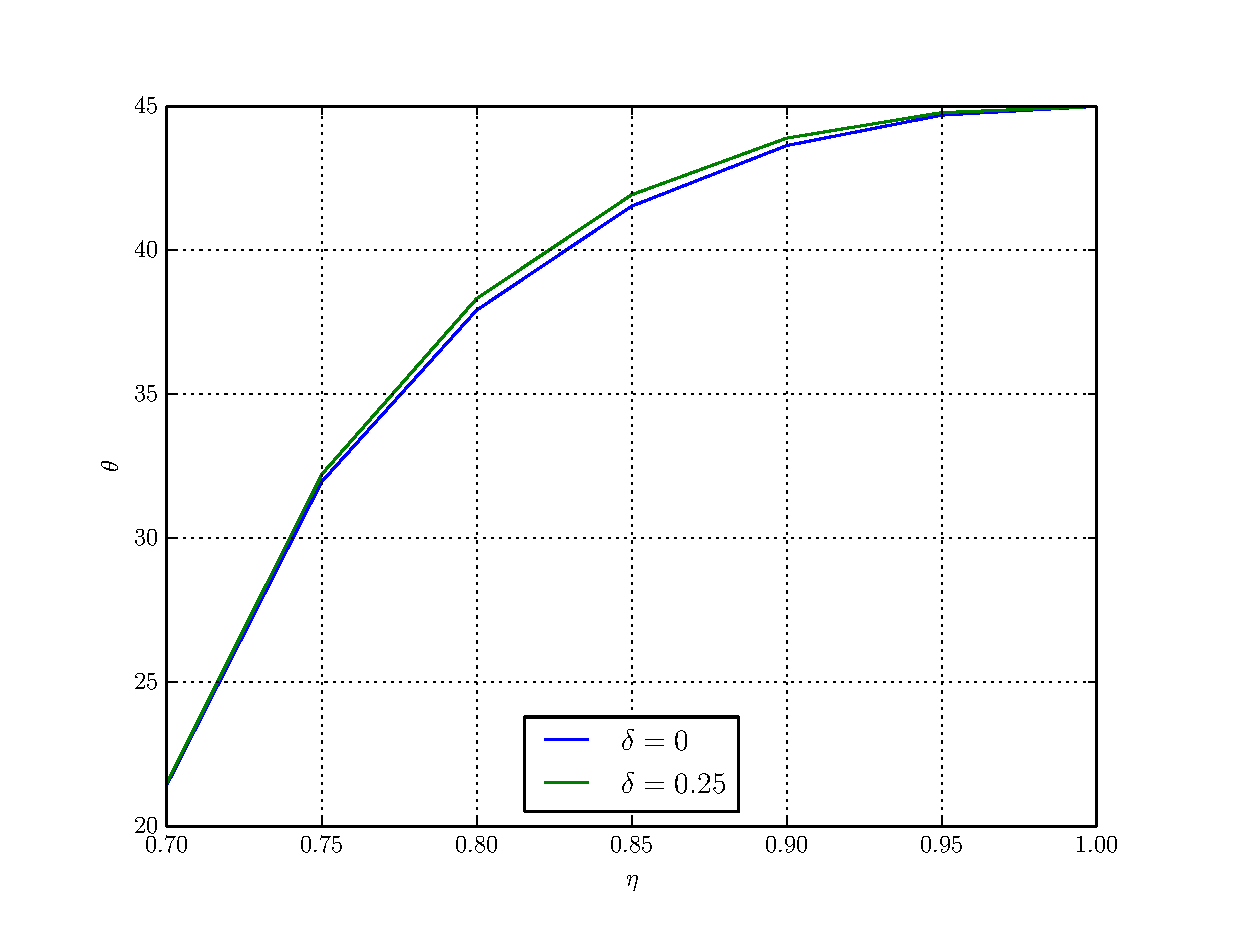
\includegraphics[scale=0.7]{theta_4ang.eps}
\caption{Оптимизированные значения для $\theta$ для различных значений углов}
\label{fig:theta_4ang}
\end{figure}

\begin{figure}[h]
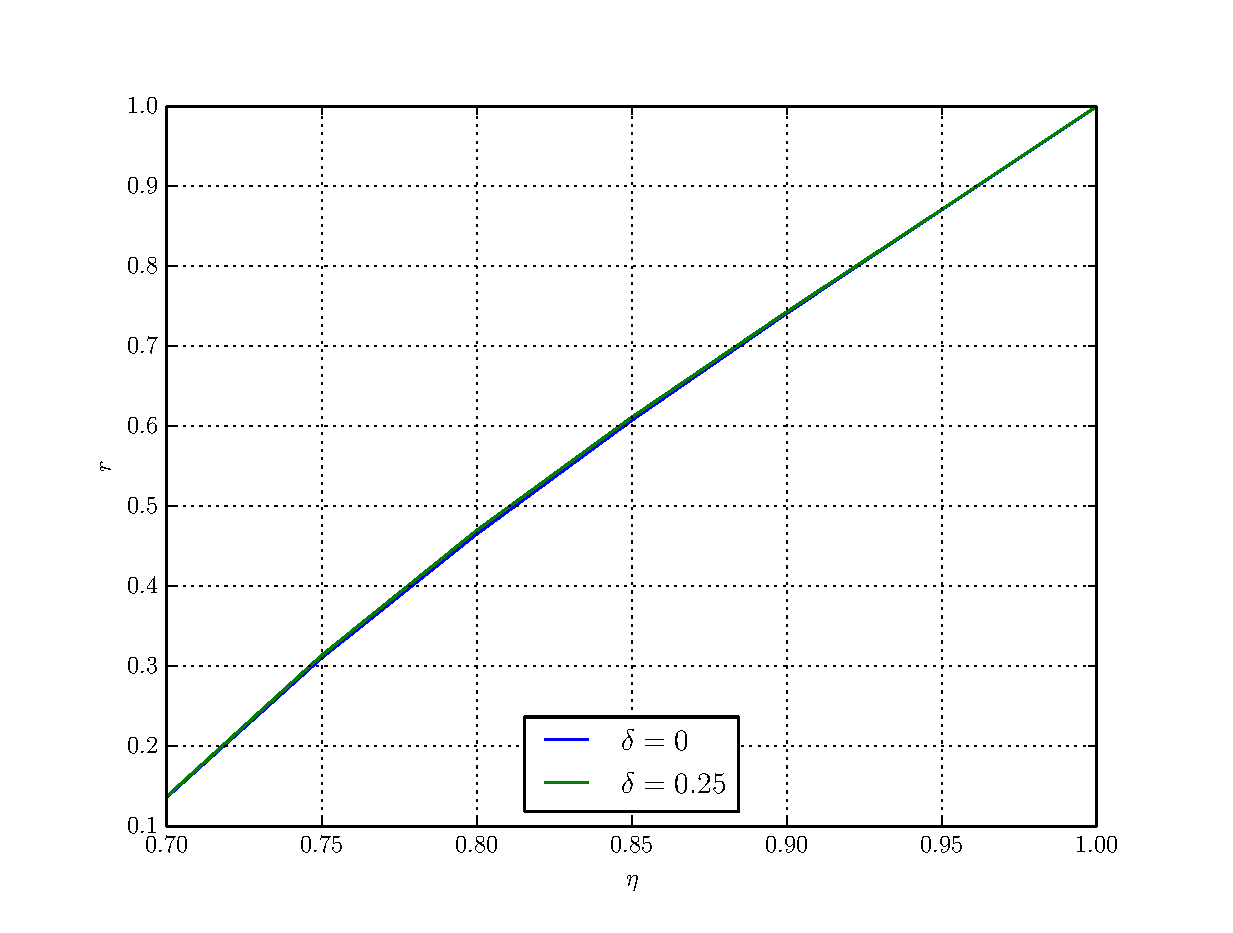
\includegraphics[scale=0.7]{r_4ang.eps}
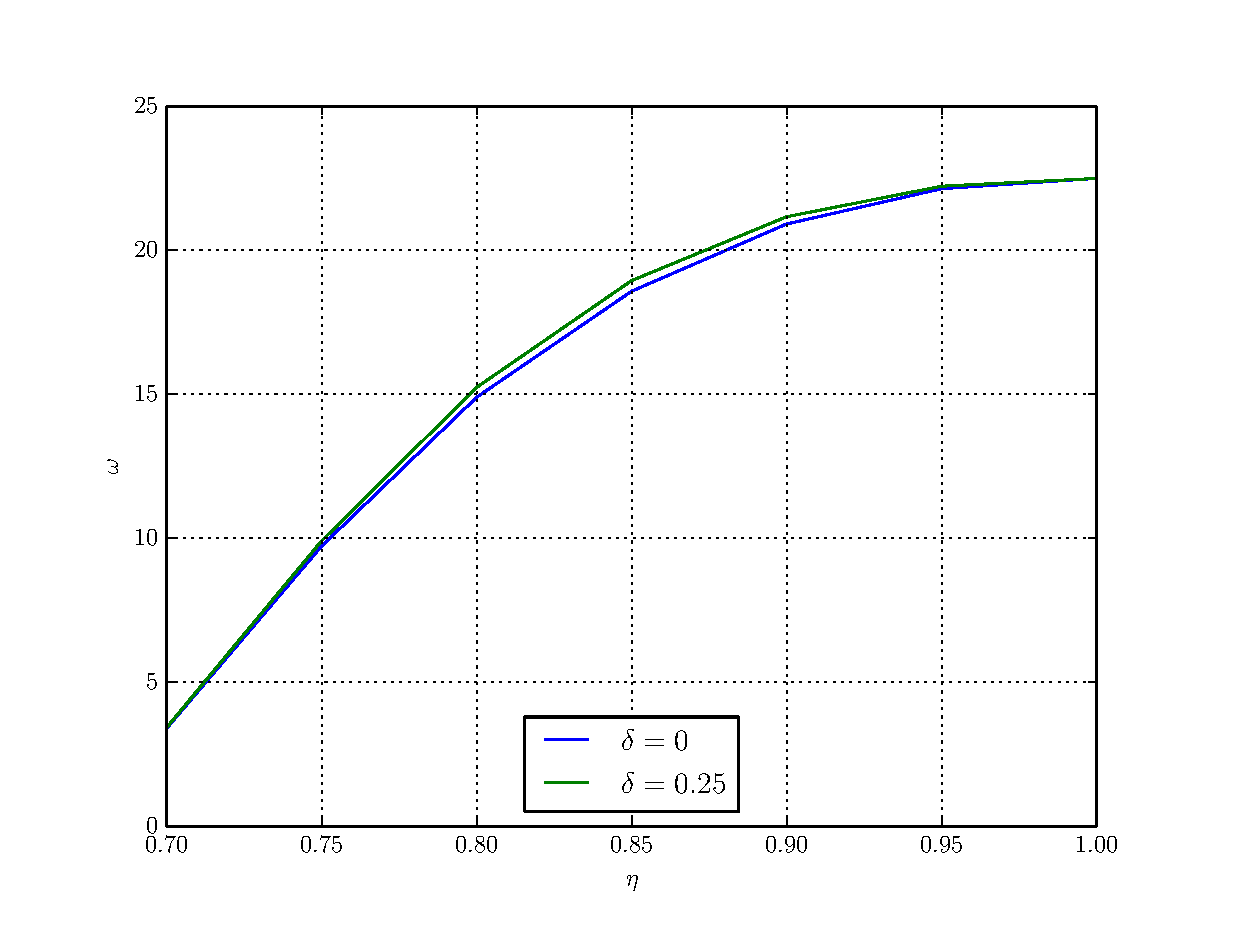
\includegraphics[scale=0.7]{omega_4ang.eps}
\caption{Оптимизированные значения для $r$ и $\omega$ для различных значений углов}
\label{fig:psi_4ang}
\end{figure}

\begin{figure}[t]
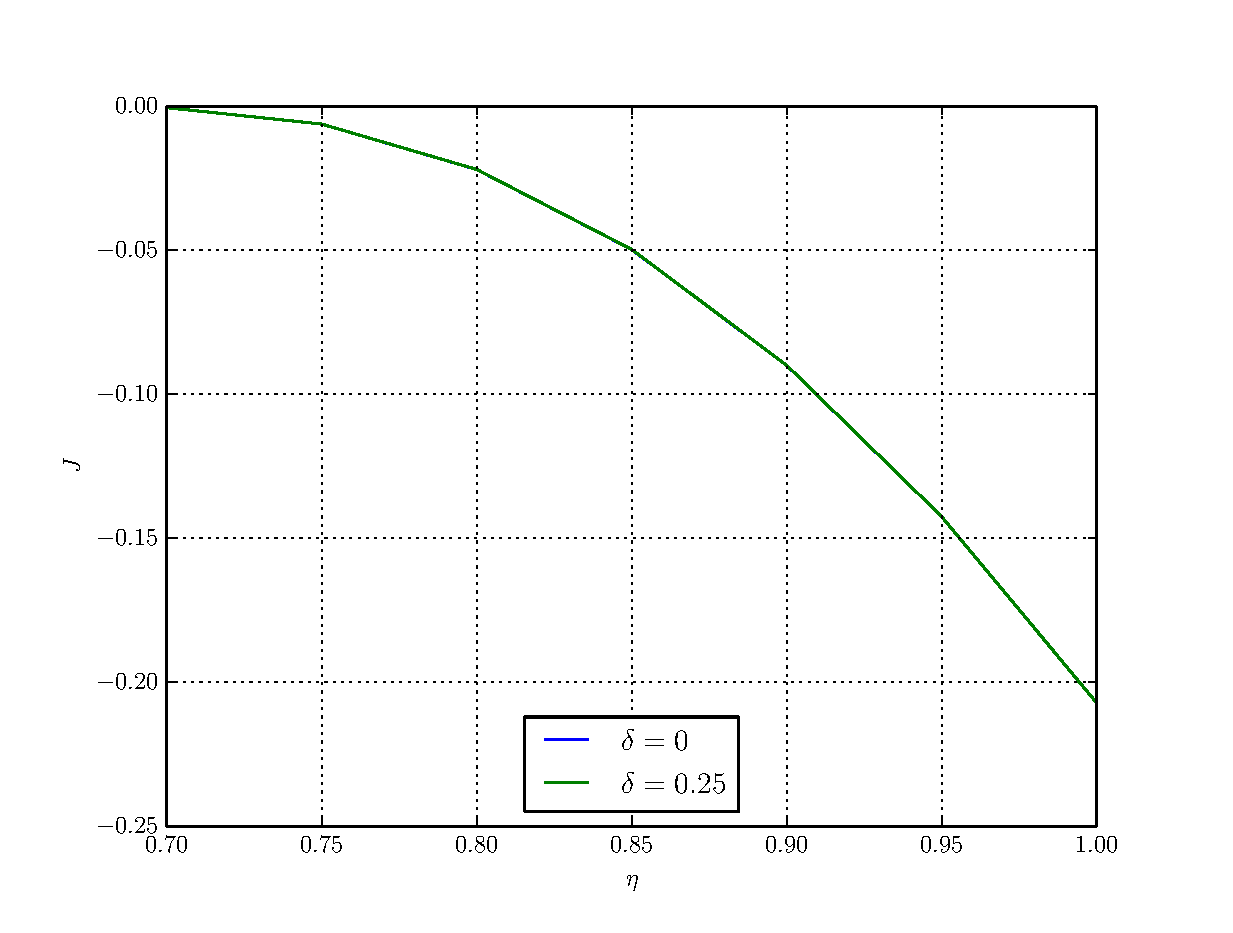
\includegraphics[scale=0.7]{K_4ang.eps}
\caption{Оптимизированные значения для $J_{\mathcal{B}}/N$ для различных значений углов}
\label{fig:J_4ang}
\end{figure}

\begin{table}
\small
\begin{tabular}{|c|c|c|c|c|c|c|c|c|}
\hline
$\eta$ & $\delta,^\circ$ & $r$ & $\omega,^\circ$ & $\theta,^\circ$ & $J$ & $J_{\delta}$ & $\sigma_{\delta}$ & $K = J_{\delta}/\sigma_{\delta}$
\\\hline
\multirow{3}{*}{0.7} & \multirow{3}{*}{0.25} & 0.136389 & 3.40081 & 21.4266 & -0.000453562 & -0.000444565 & 0.00241554 & -0.184044\\\cline{3-9}
 &  & 0.136389 & 3.40081 & 21.4266 & -0.000453562 & -0.000444565 & 0.00241554 & -0.184044\\\cline{3-9}
 &  & 0.137124 & 3.42997 & 21.496 & -0.000453514 & -0.000444515 & 0.00241503 & -0.184062\\\hline
 \multirow{3}{*}{0.75} & \multirow{3}{*}{0.25} & 0.310518 & 9.73143 & 31.9603 & -0.00615095 & -0.00614082 & 0.00248895 & -2.46724\\\cline{3-9}
 &  & 0.310518 & 9.73143 & 31.9603 & -0.00615095 & -0.00614082 & 0.00248895 & -2.46724\\\cline{3-9}
 &  & 0.313658 & 9.91344 & 32.2158 & -0.00614786 & -0.00613773 & 0.00248642 & -2.4685\\\hline
\multirow{3}{*}{0.8} & \multirow{3}{*}{0.25} & 0.465228 & 14.8979 & 37.9215 & -0.02191 & -0.0218985 & 0.002596 & -8.43546\\\cline{3-9}
 &  & 0.465228 & 14.8979 & 37.9215 & -0.02191 & -0.0218985 & 0.002596 & -8.43546\\\cline{3-9}
 &  & 0.469841 & 15.2419 & 38.3231 & -0.0218953 & -0.0218838 & 0.00259252 & -8.44116\\\hline
\multirow{3}{*}{0.85} & \multirow{3}{*}{0.25} & 0.607424 & 18.5808 & 41.5341 & -0.0496902 & -0.0496772 & 0.00275221 & -18.0499\\\cline{3-9}
 &  & 0.607424 & 18.5808 & 41.5341 & -0.0496902 & -0.0496772 & 0.00275221 & -18.0499\\\cline{3-9}
 &  & 0.61123 & 18.9498 & 41.9292 & -0.0496699 & -0.0496569 & 0.00274992 & -18.0576\\\hline
\multirow{3}{*}{0.9} & \multirow{3}{*}{0.25} & 0.741202 & 20.9153 & 43.6381 & -0.0899078 & -0.0898932 & 0.00296469 & -30.3213\\\cline{3-9}
 &  & 0.741202 & 20.9153 & 43.6381 & -0.0899078 & -0.0898932 & 0.00296469 & -30.3213\\\cline{3-9}
 &  & 0.743038 & 21.167 & 43.8961 & -0.0898969 & -0.0898824 & 0.00296395 & -30.3252\\\hline
\multirow{3}{*}{0.95} & \multirow{3}{*}{0.25} & 0.87067 & 22.141 & 44.6958 & -0.142436 & -0.14242 & 0.00323493 & -44.0258\\\cline{3-9}
 &  & 0.87067 & 22.141 & 44.6958 & -0.142436 & -0.14242 & 0.00323493 & -44.0258\\\cline{3-9}
 &  & 0.871004 & 22.2272 & 44.7823 & -0.142435 & -0.142419 & 0.00323486 & -44.0263\\\hline
\multirow{3}{*}{1.0} & \multirow{3}{*}{0.25} & 0.999997 & 22.5 & 45 & -0.207107 & -0.207089 & 0.0035626 & -58.1286\\\cline{3-9}
 &  & 0.999997 & 22.5 & 45 & -0.207107 & -0.207089 & 0.0035626 & -58.1286\\\cline{3-9}
 &  & 0.999999 & 22.4981 & 44.998 & -0.207107 & -0.207089 & 0.0035626 & -58.1286\\\hline
 \end{tabular}
\caption{Значения оптимизированных параметров для погрешности в четырех углах в отдельности для случай $\delta = 0.25^\circ$}
\label{tab:different_deltas}
\end{table}


Результаты проведенной оптимизации представлены на рисунках \ref{fig:theta_4ang} - \ref{fig:J_4ang} и в таблице \ref{tab:different_deltas}, строки которой также сгруппированы по три. Из графиков видно, что добавление разброса почти не изменяет оптимальные параметры. А это означает, что можно сделать предположение, что контроль за величиной углов детекторов можно уменьшить. 

\bibliography{literature.bib}
\bibliographystyle{ieeetr}
\end{document}